\chapter{La Carretera Austral}
\section*{28 février 2015}
Retour sur le continent chilien après l'île de Chiloe pour emprunter une partie de la Carretera Austral, superbe route qui traverse la Patagonie chilienne sur plus de 1000km. \newline
 J'avais prévu d'en faire environ 700km mais j'ai du changer mes plans à cause du ferry que je n'ai pas pu avoir plus tôt. \newline
 Le ferry m'a donc amené à Puerto Raul Marin Balmaceda, un tout petit village où pas grand monde ne va. \newline
 \newline
\centerline{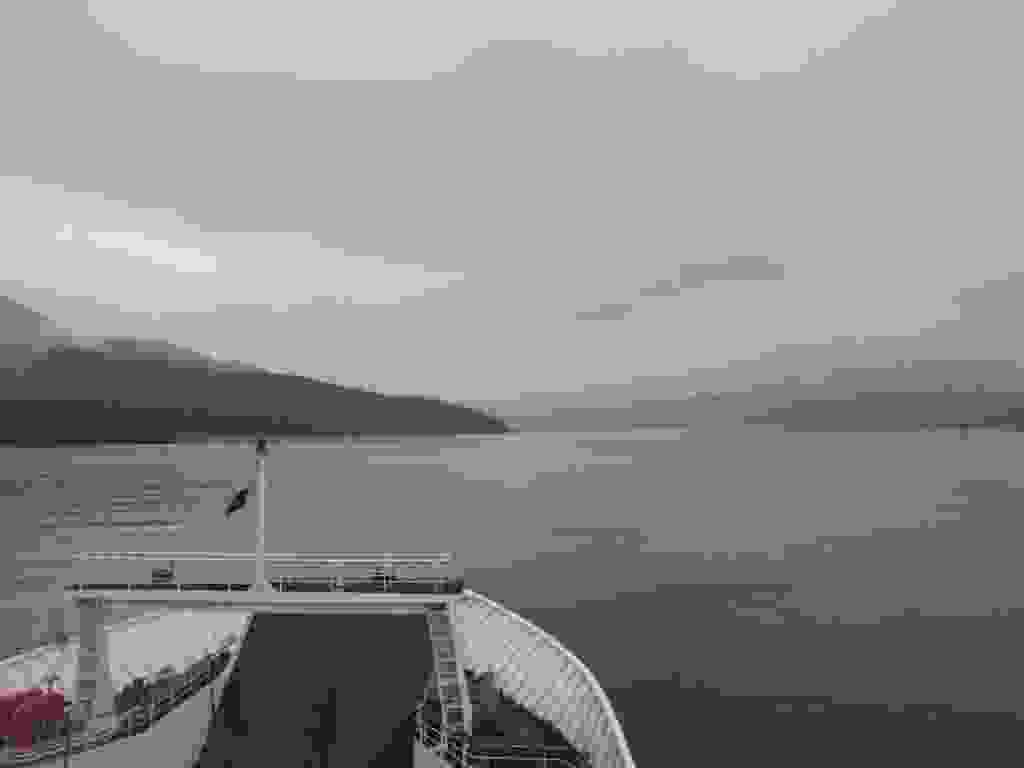
\includegraphics[height=90mm]{../wp-content/uploads/2015/02/P2192198.jpg} } 
\newline
\centerline{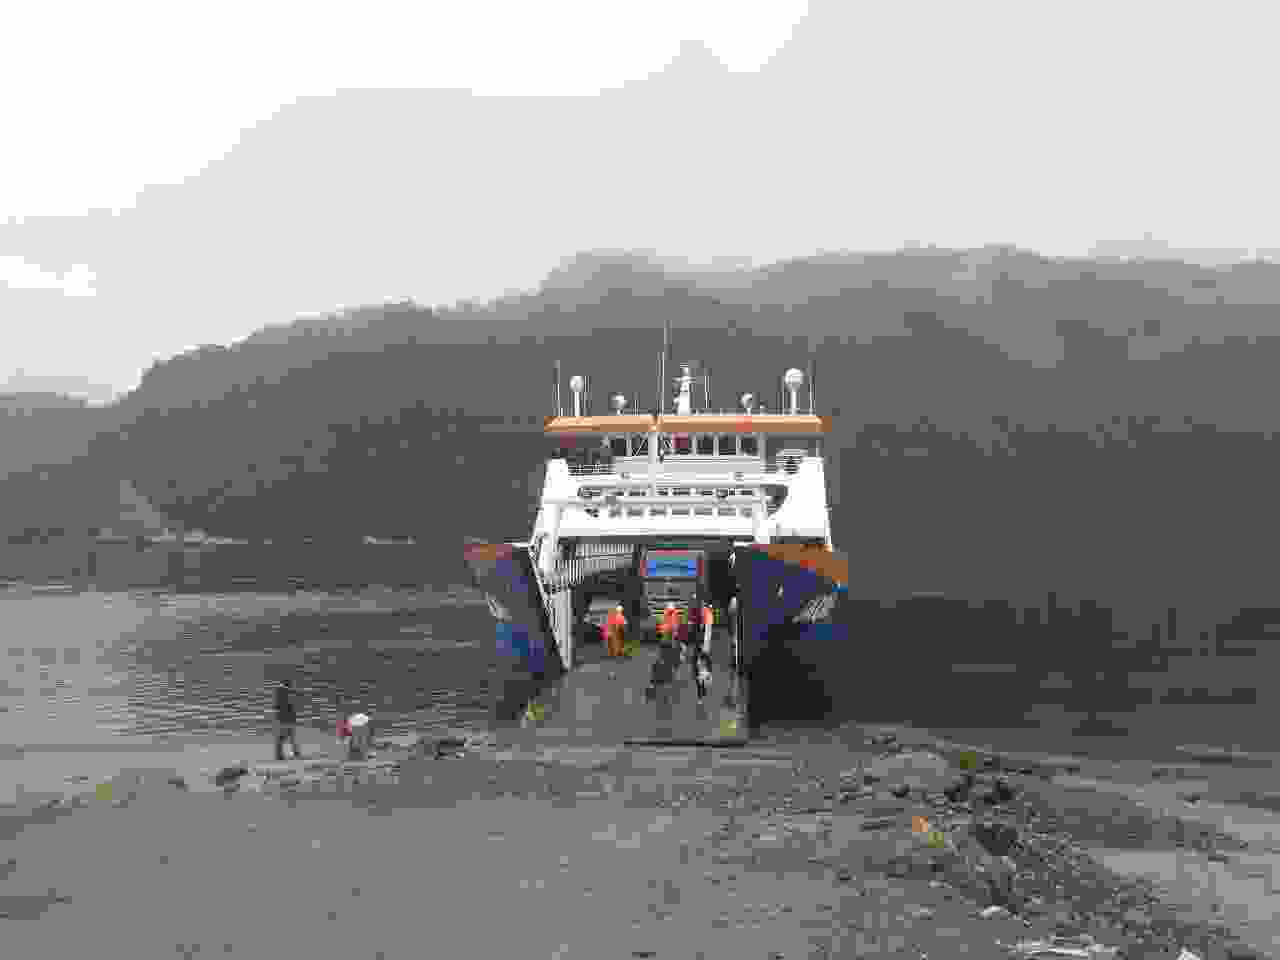
\includegraphics[height=90mm]{../wp-content/uploads/2015/02/P2192200.jpg} } 
 \newline
\centerline{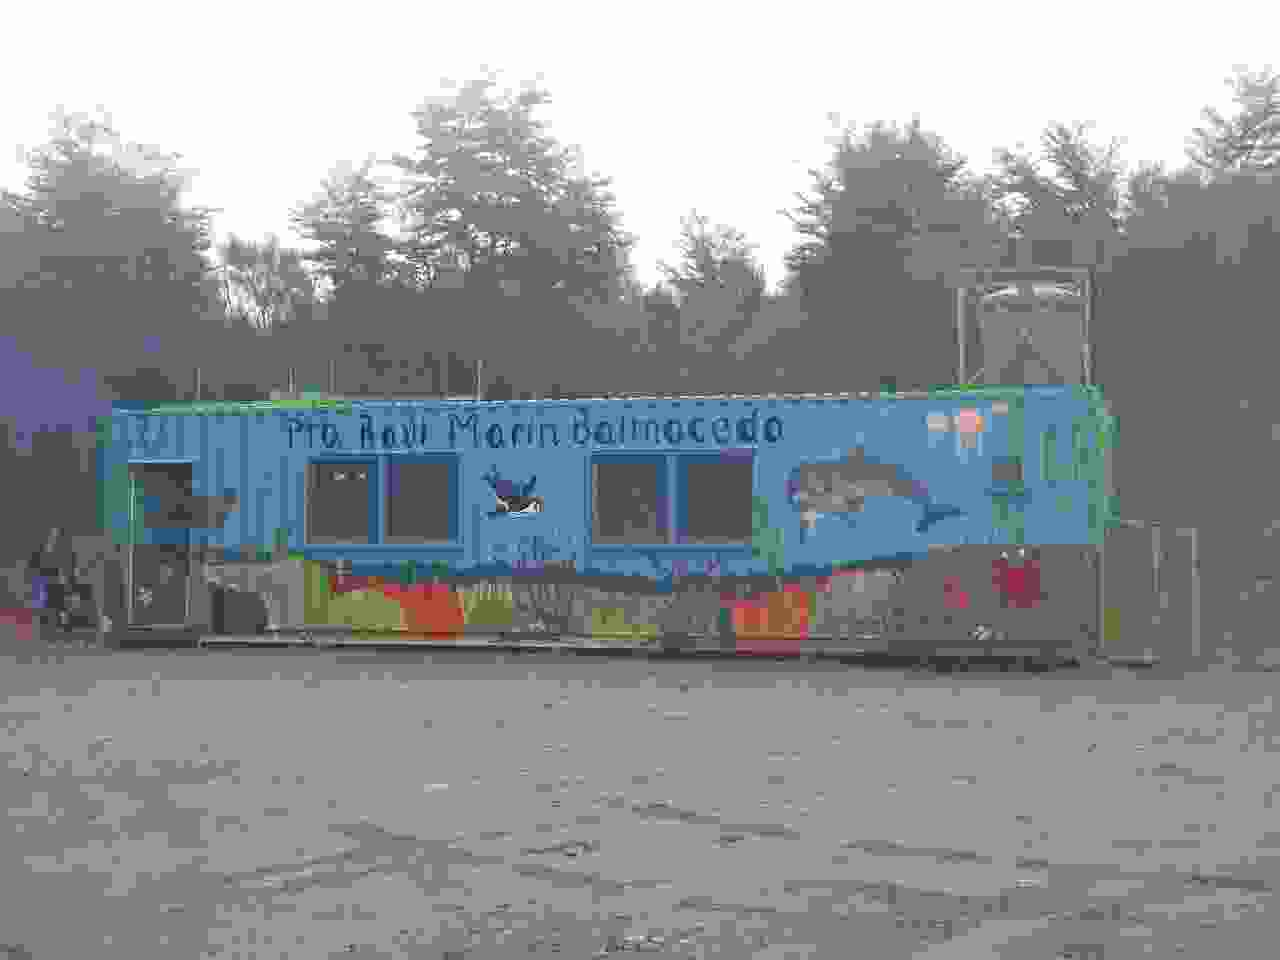
\includegraphics[height=90mm]{../wp-content/uploads/2015/02/P2192201.jpg} } 
70km de piste pour rejoindre la Carretera Austral, le long de la belle rivière Palena. \newline
 \newline
\centerline{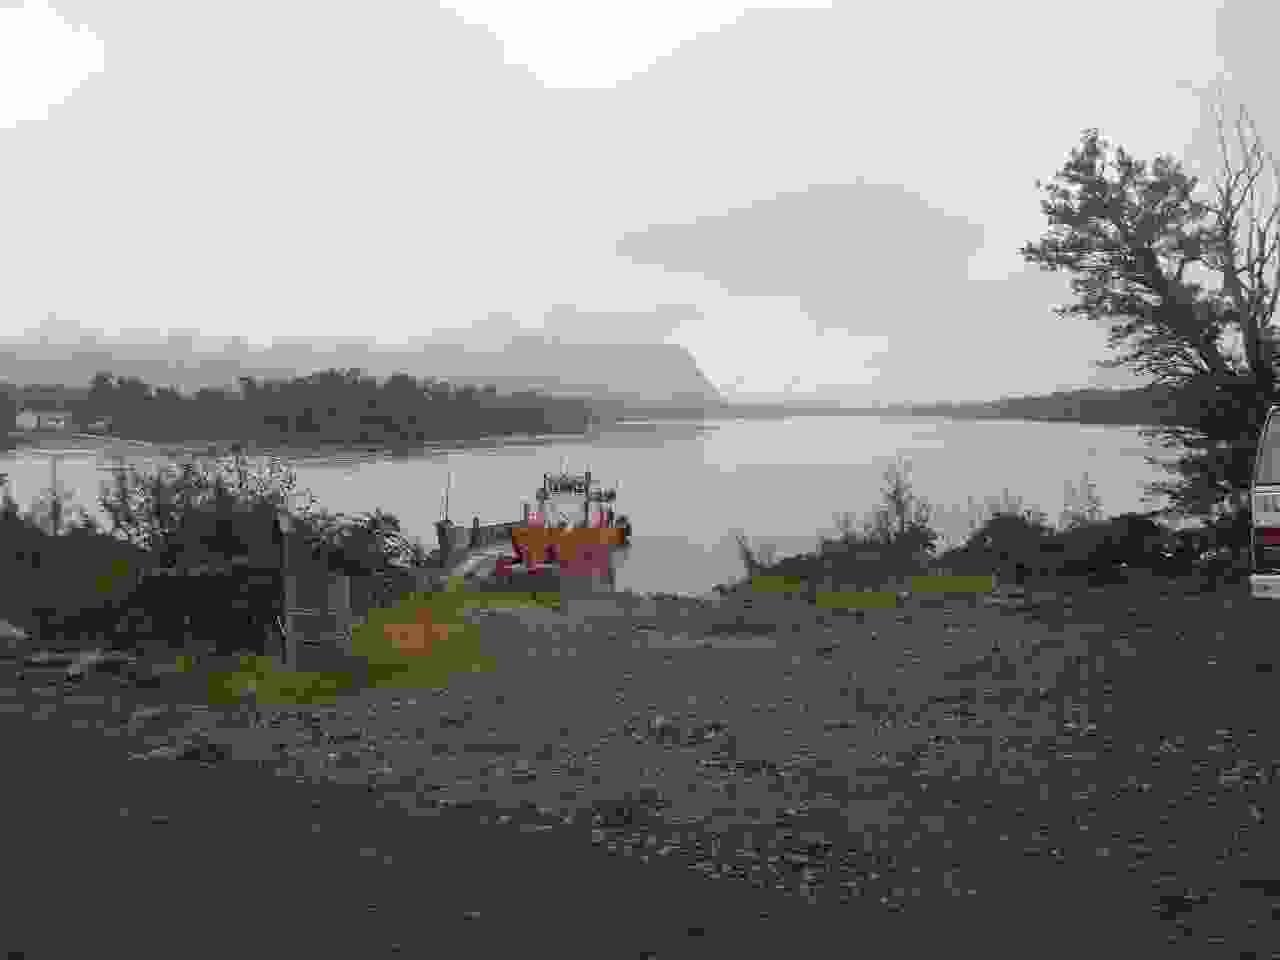
\includegraphics[height=90mm]{../wp-content/uploads/2015/02/P2192214.jpg} } 
 \newline
\centerline{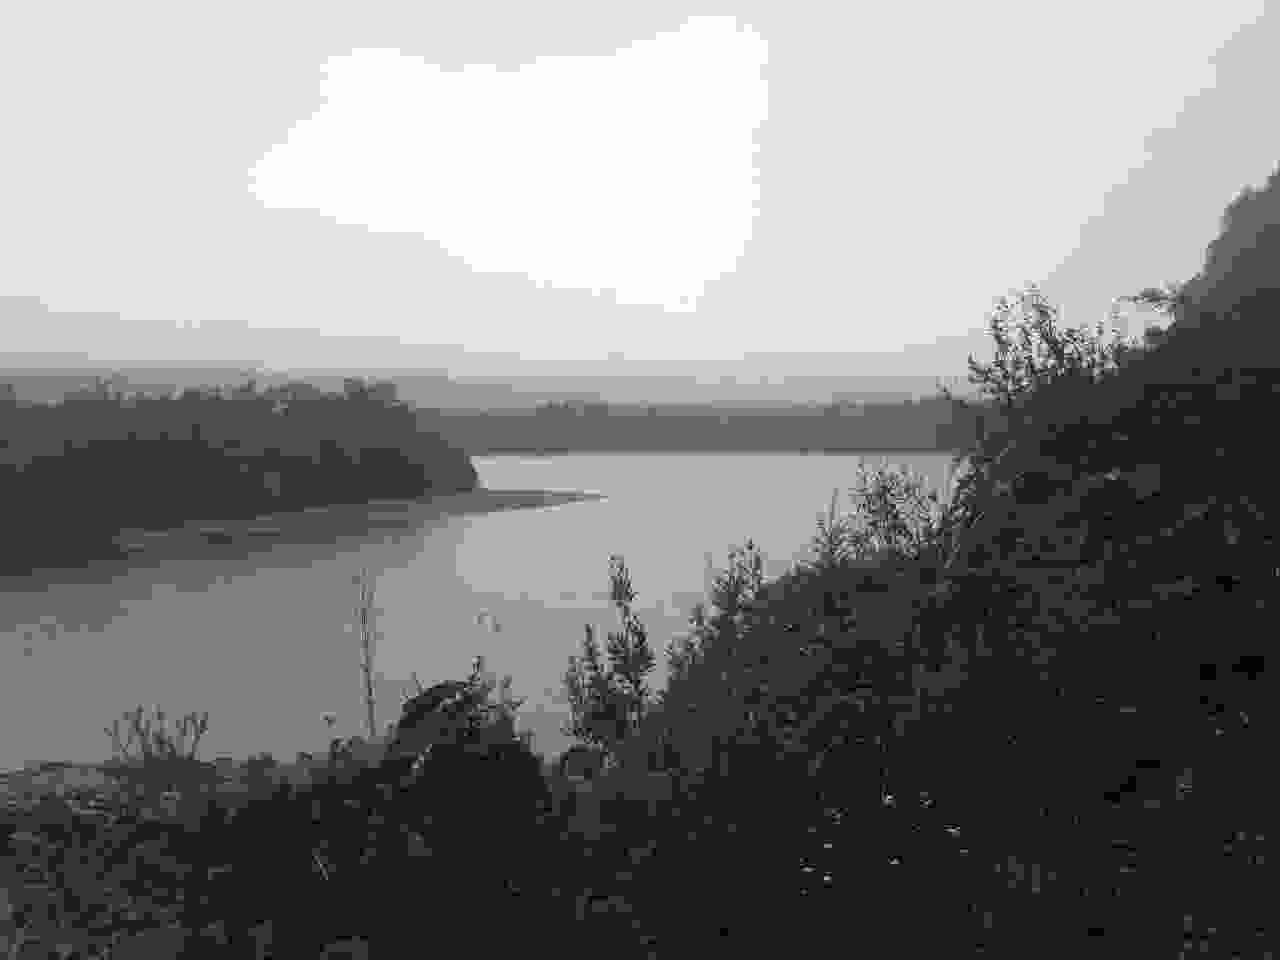
\includegraphics[height=90mm]{../wp-content/uploads/2015/02/P2192216.jpg} } 
 \newline
\centerline{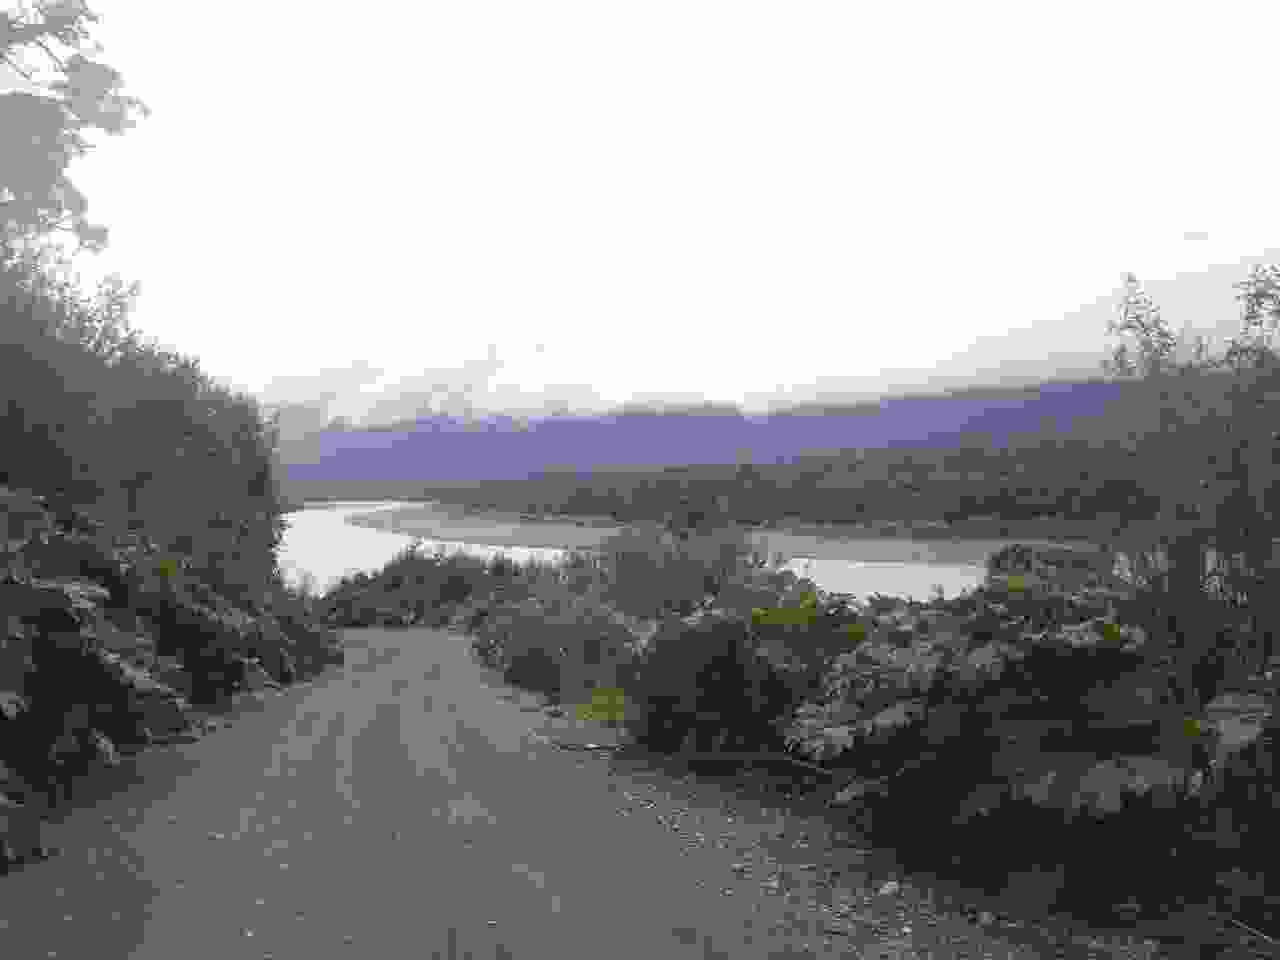
\includegraphics[height=90mm]{../wp-content/uploads/2015/02/P2192220.jpg} } 
 \newline
\centerline{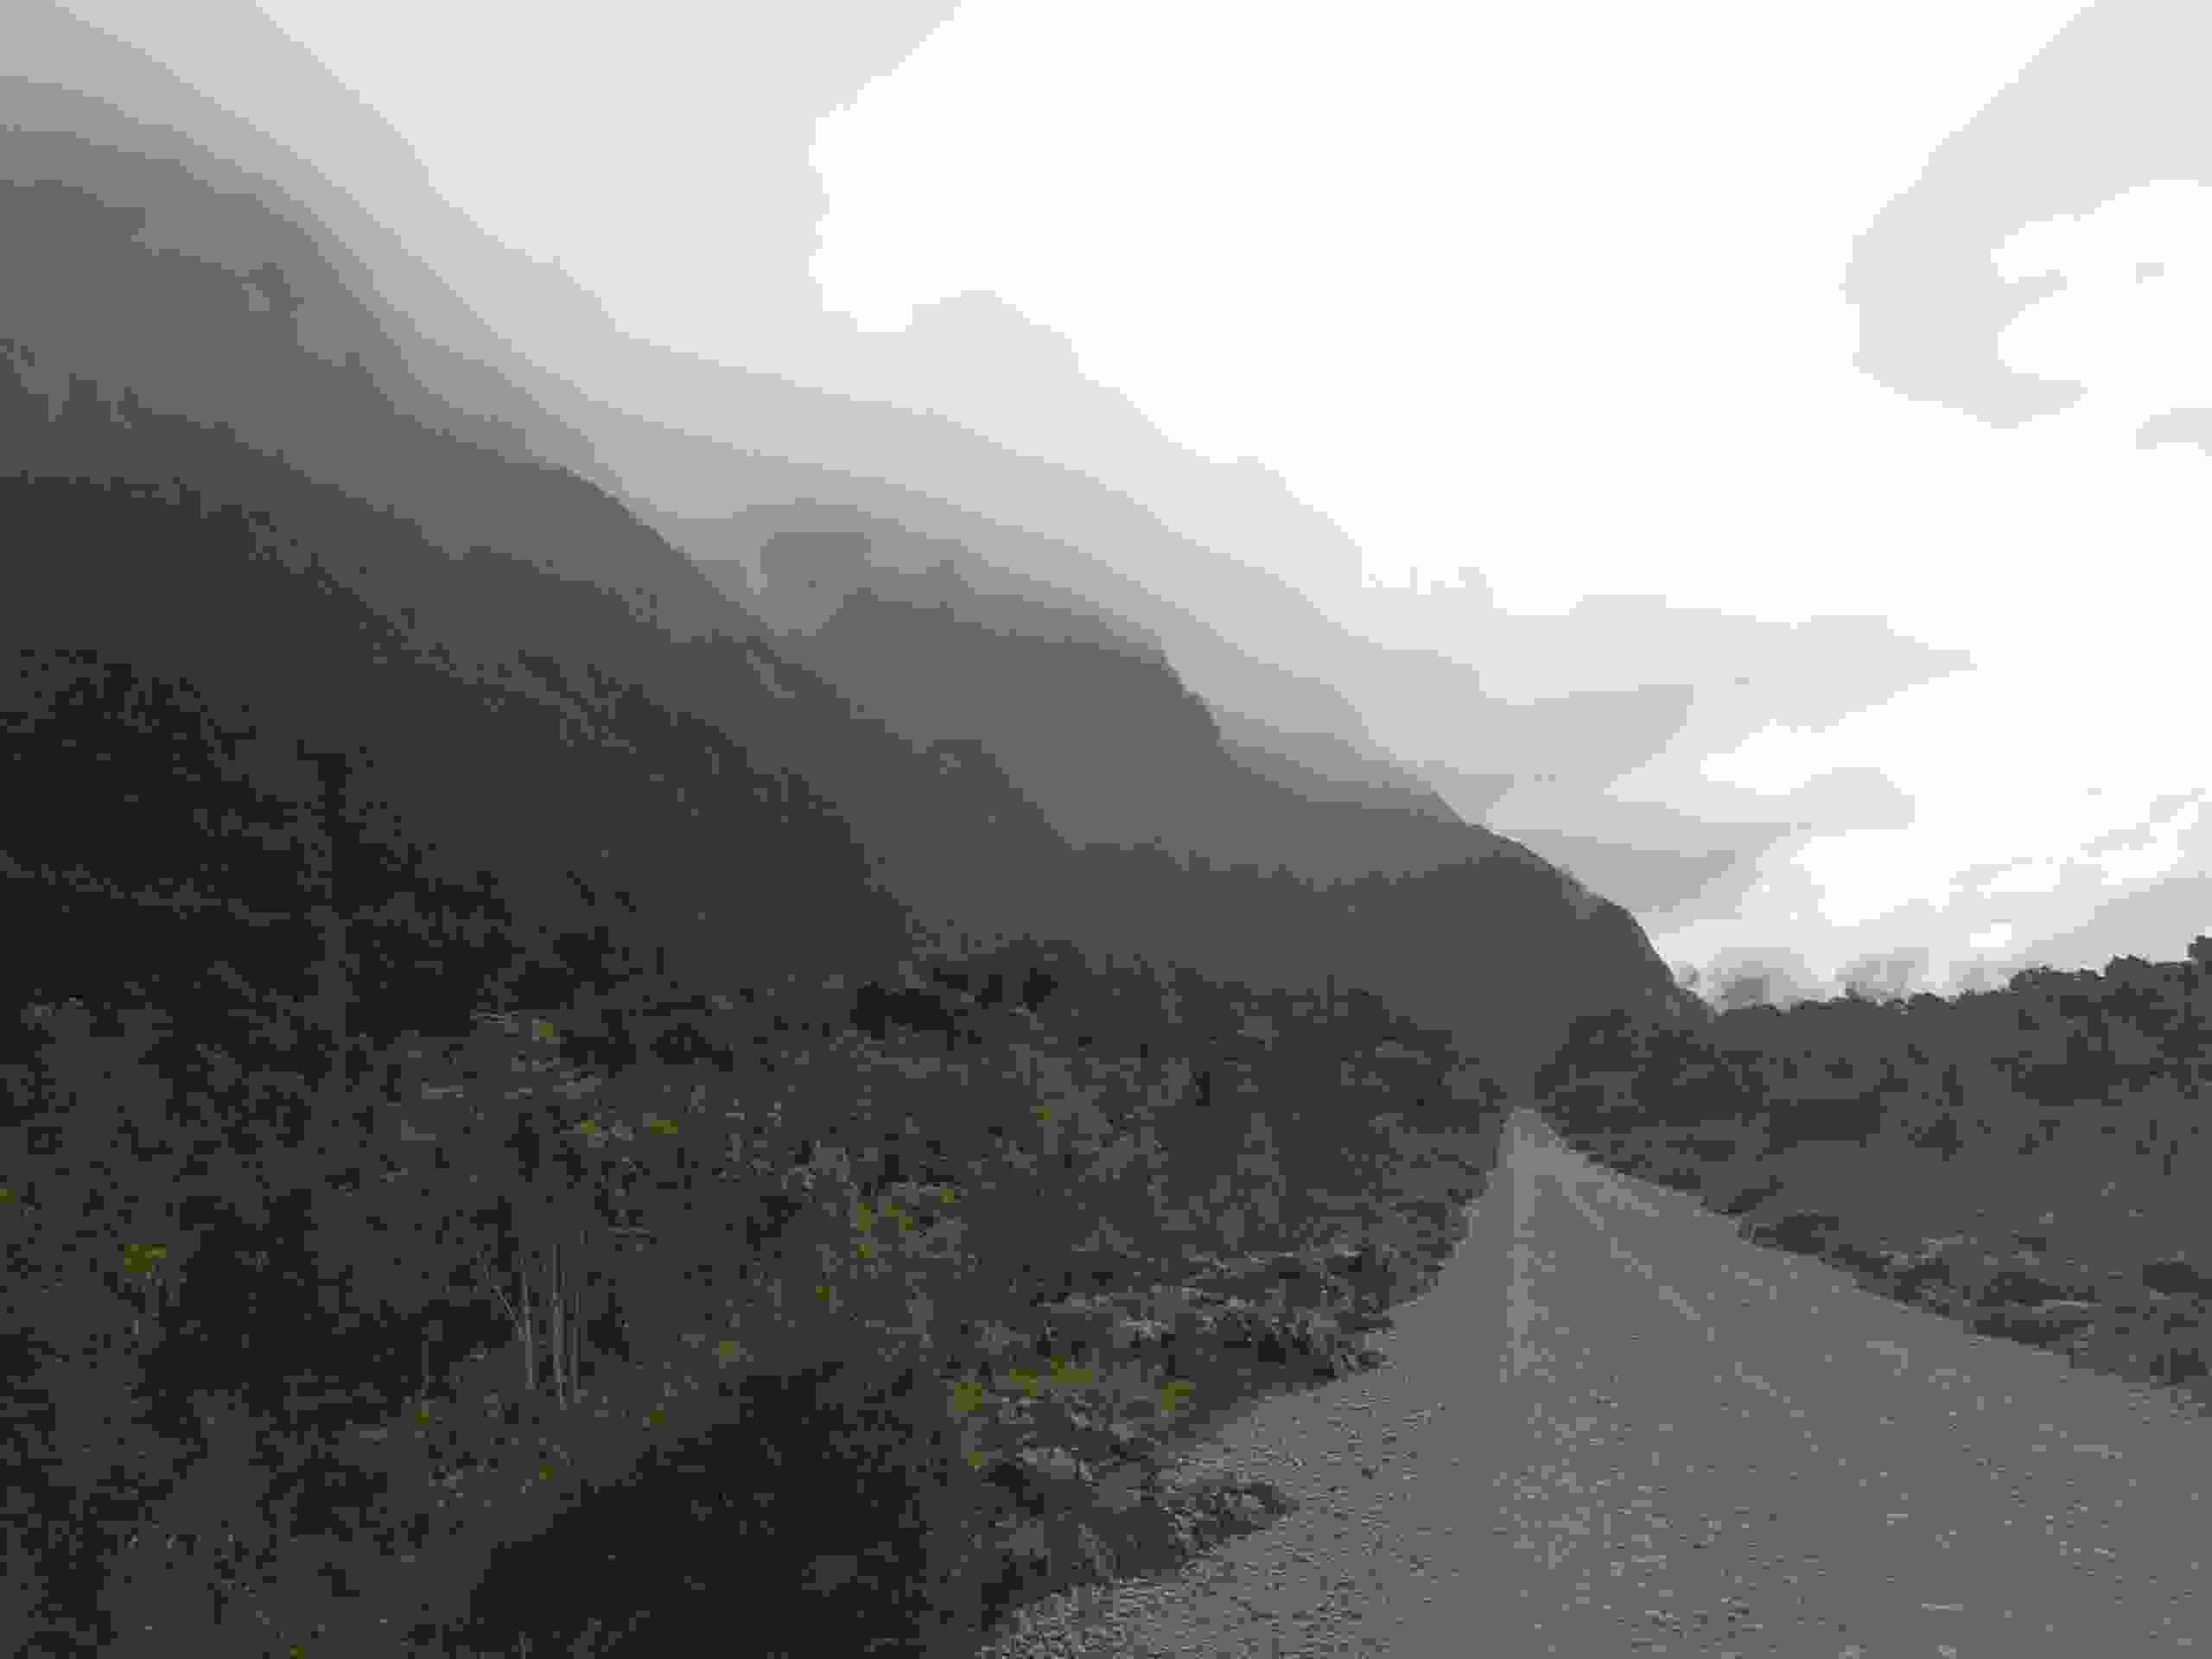
\includegraphics[height=90mm]{../wp-content/uploads/2015/02/P2192227.jpg} } 
 \newline
 Superbe bivouac au bord de l'eau.\newline
\centerline{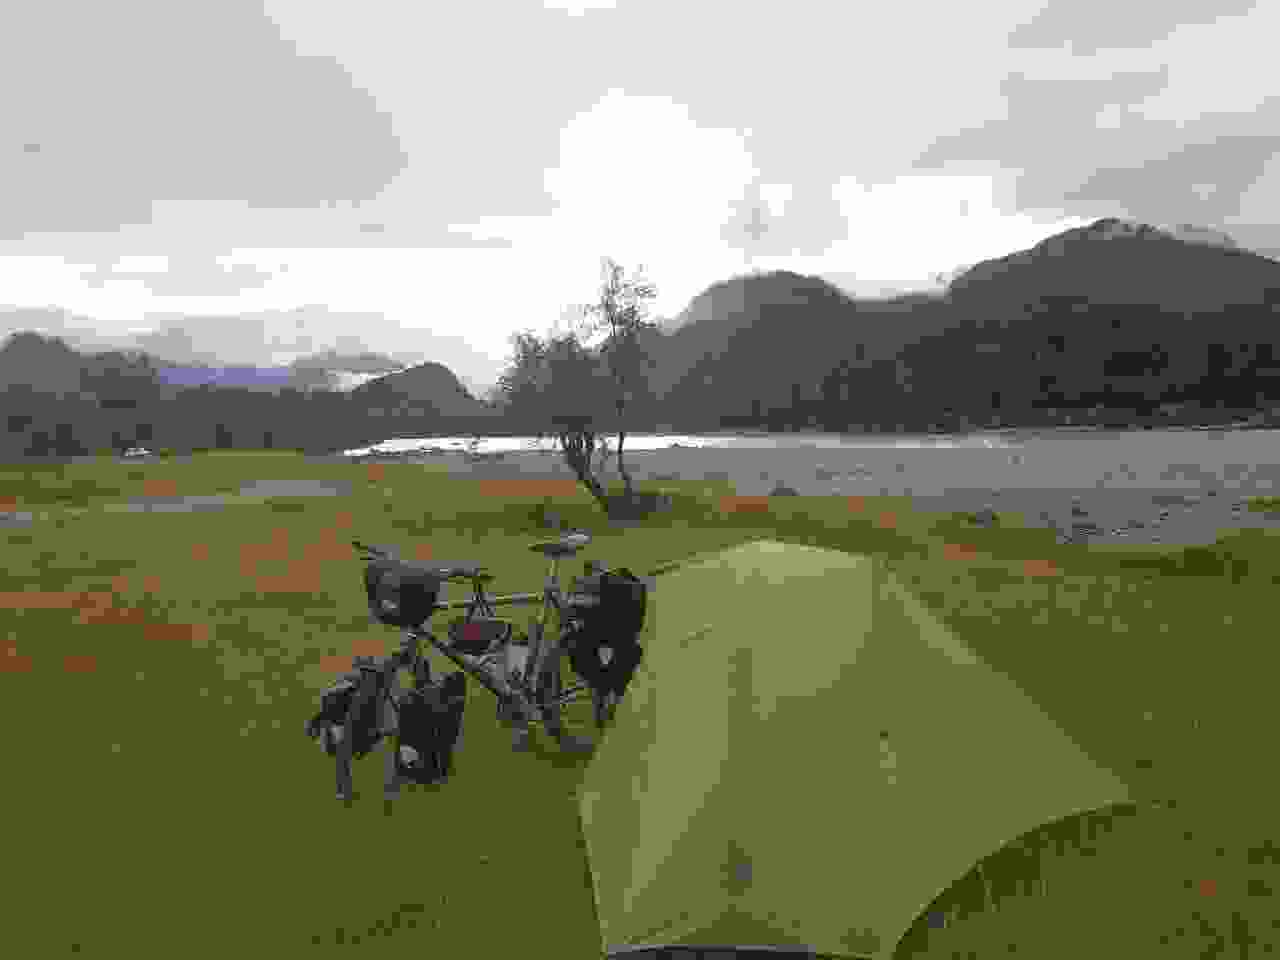
\includegraphics[height=90mm]{../wp-content/uploads/2015/02/P2202230.jpg} } 
 \newline
 \newline
\centerline{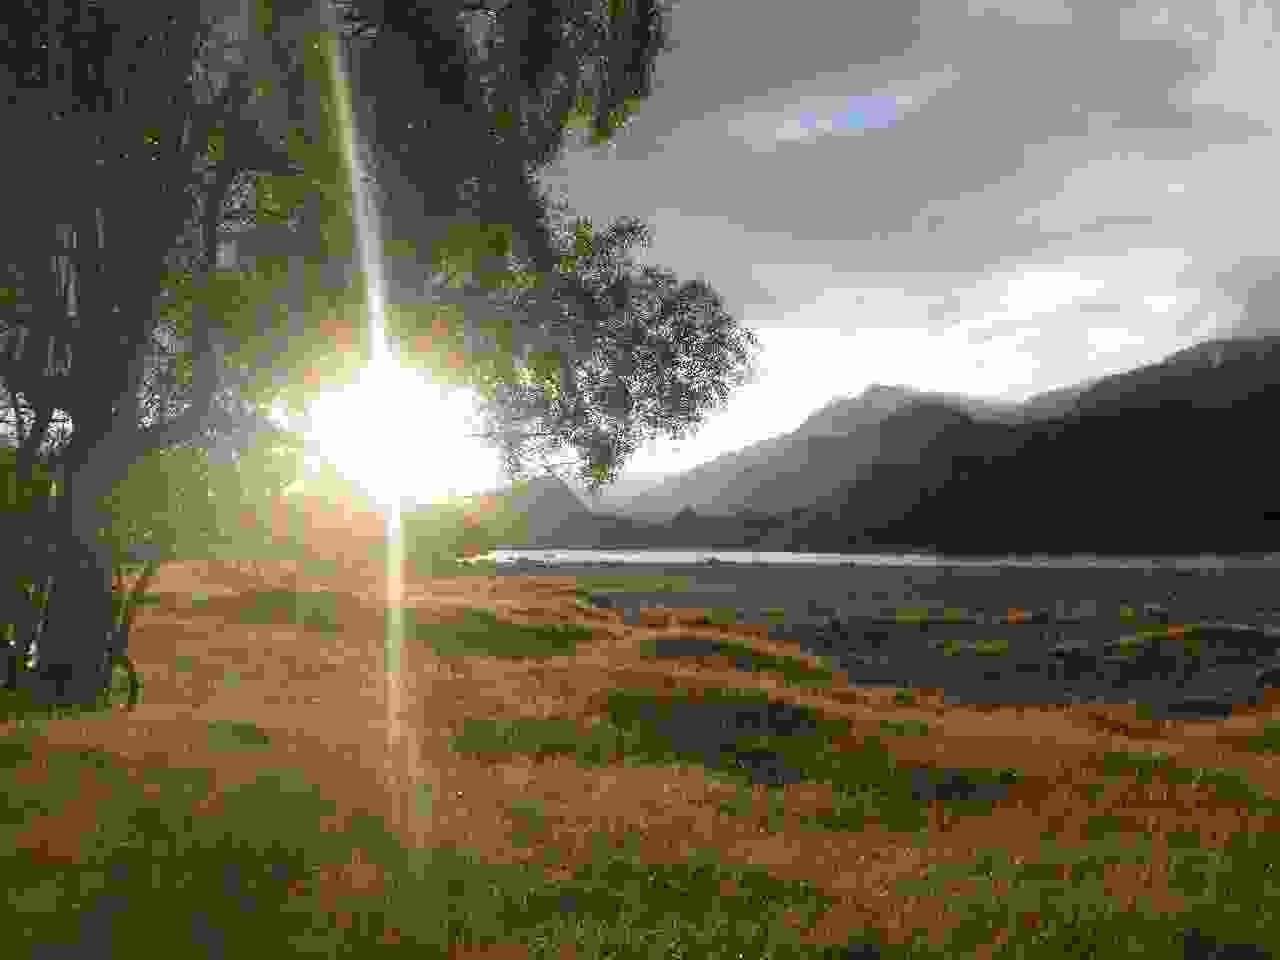
\includegraphics[height=90mm]{../wp-content/uploads/2015/02/P2202236.jpg} } 
 \newline
\centerline{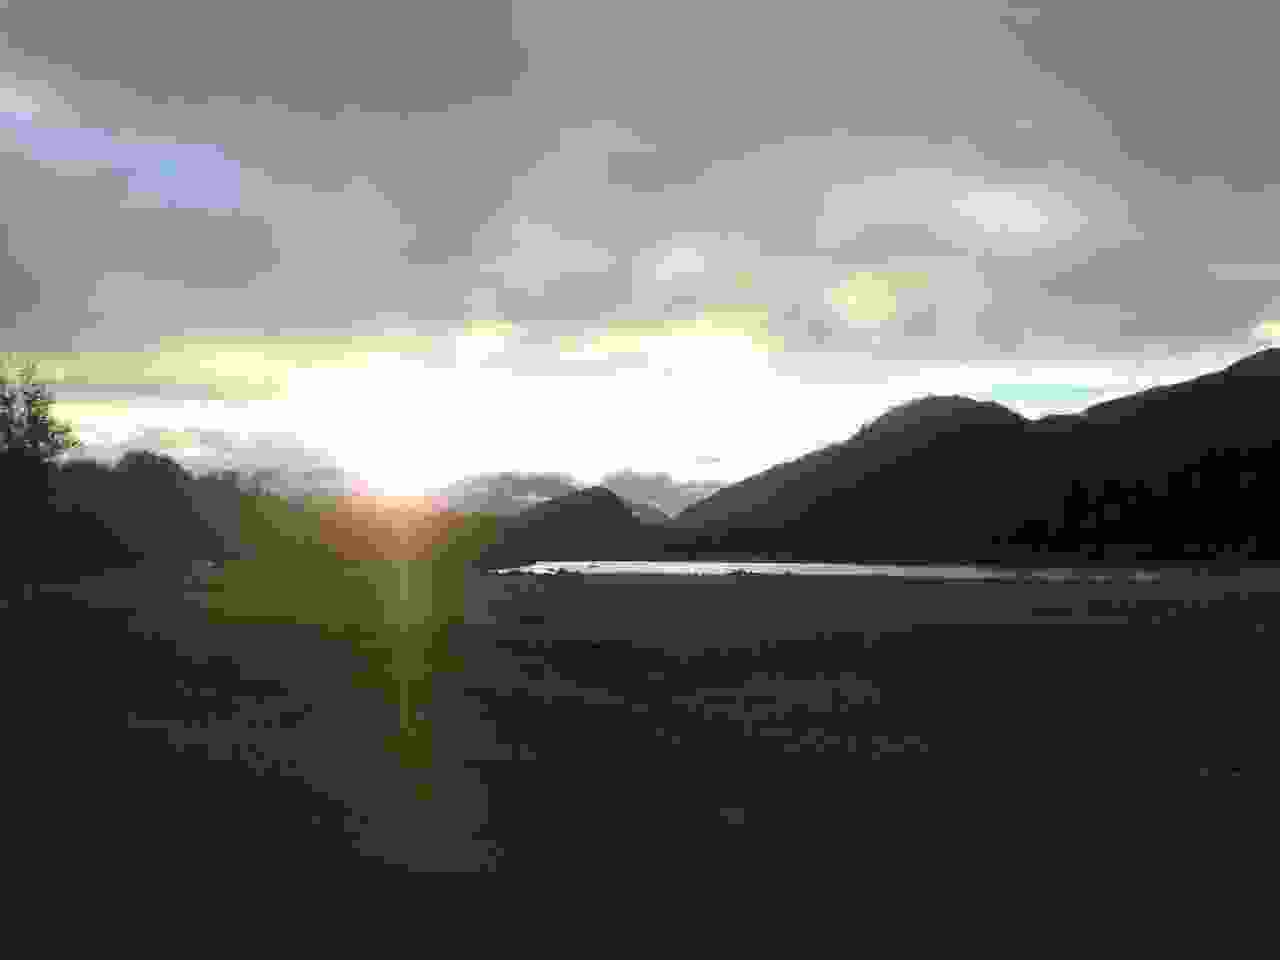
\includegraphics[height=90mm]{../wp-content/uploads/2015/02/P2202242.jpg} } 
\newline
\centerline{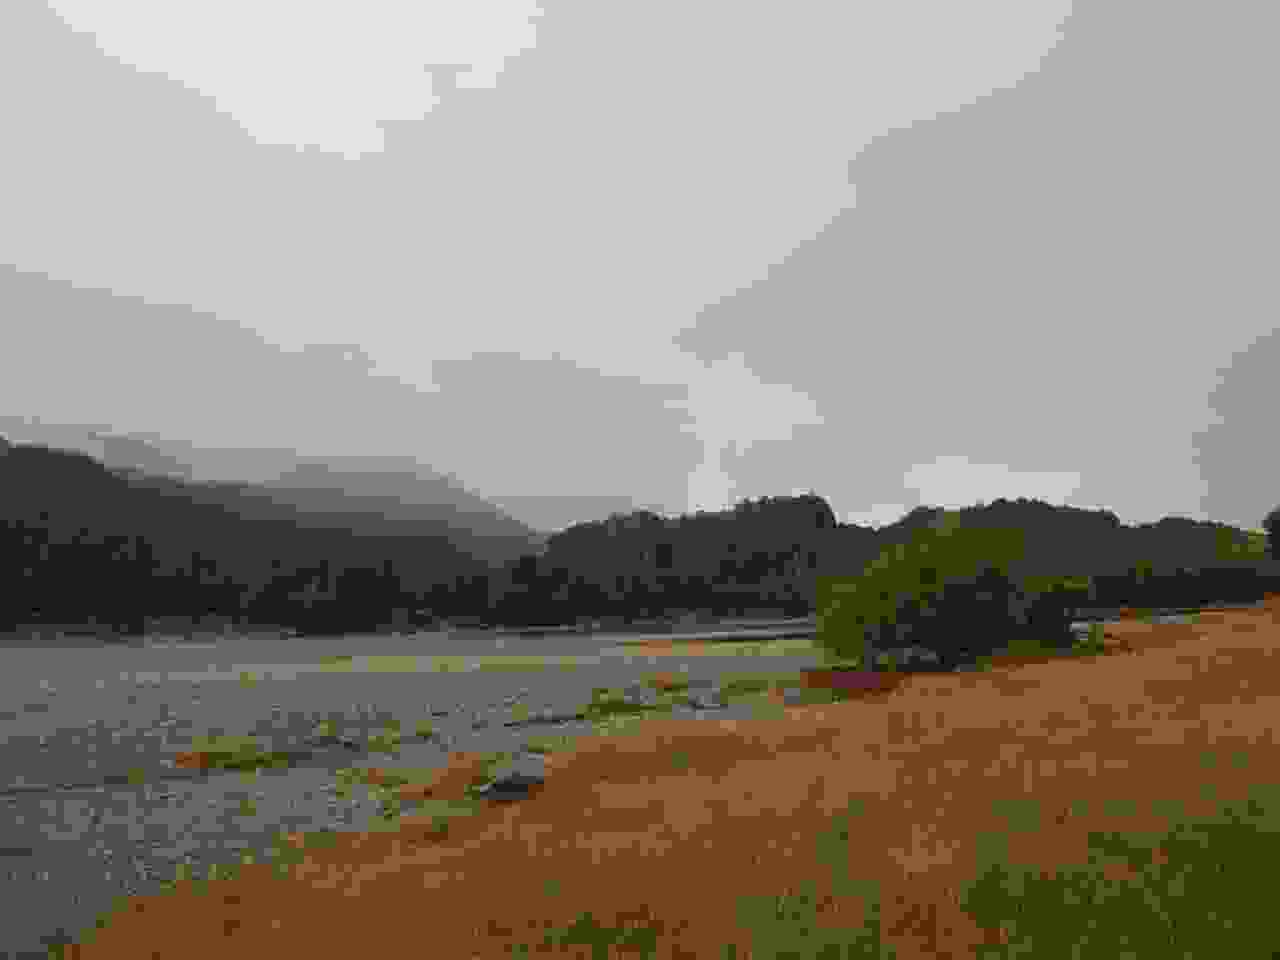
\includegraphics[height=90mm]{../wp-content/uploads/2015/02/P22022451.jpg} } 
 \newline
\centerline{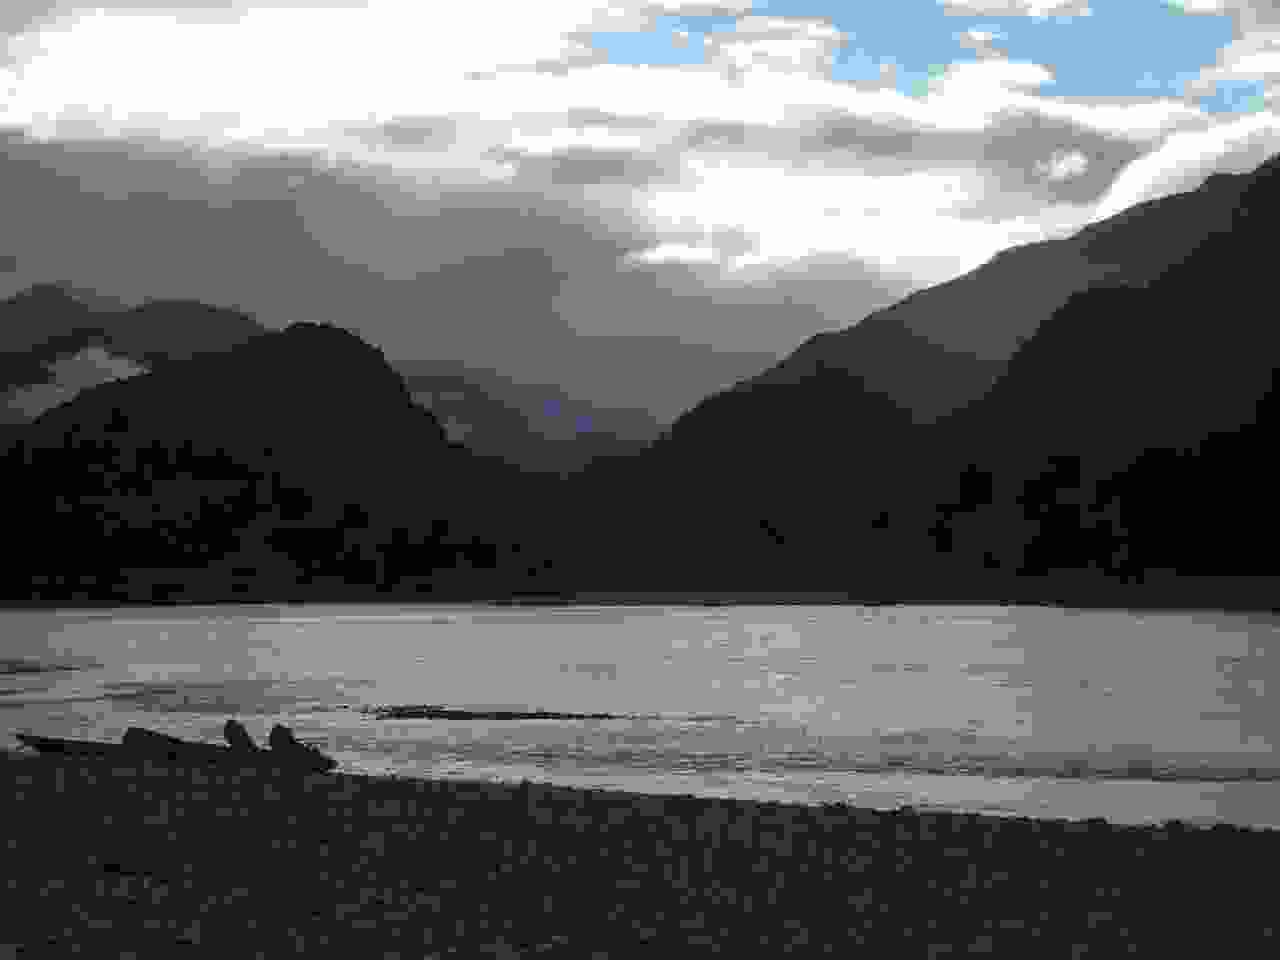
\includegraphics[height=90mm]{../wp-content/uploads/2015/02/P2202234.jpg} } 
Première étape sur la Carretera entre La Junta et Villa Santa Lucia. \newline
 \newline
\centerline{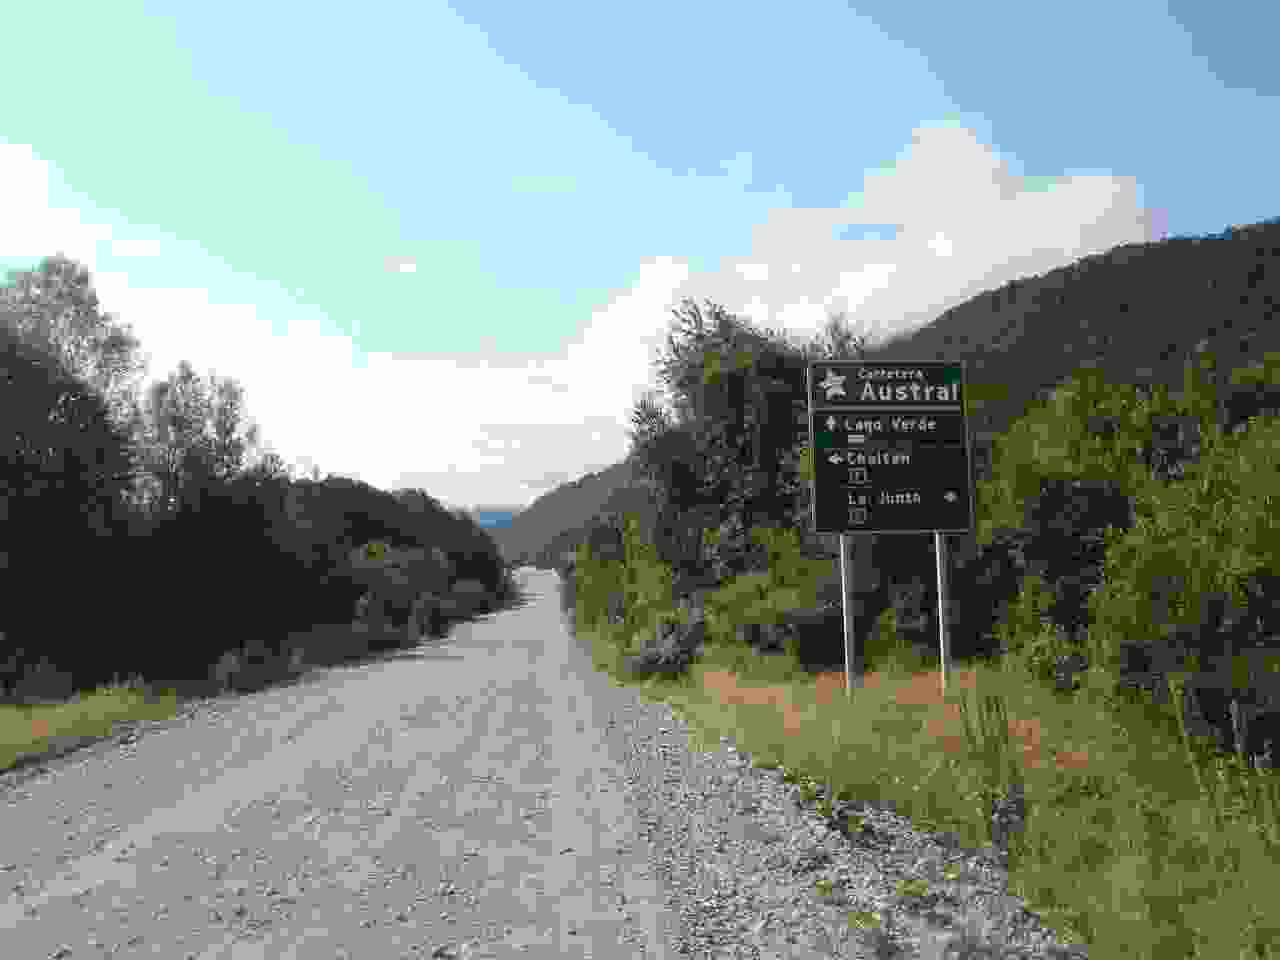
\includegraphics[height=90mm]{../wp-content/uploads/2015/02/P2202251.jpg} } 
\newline
\centerline{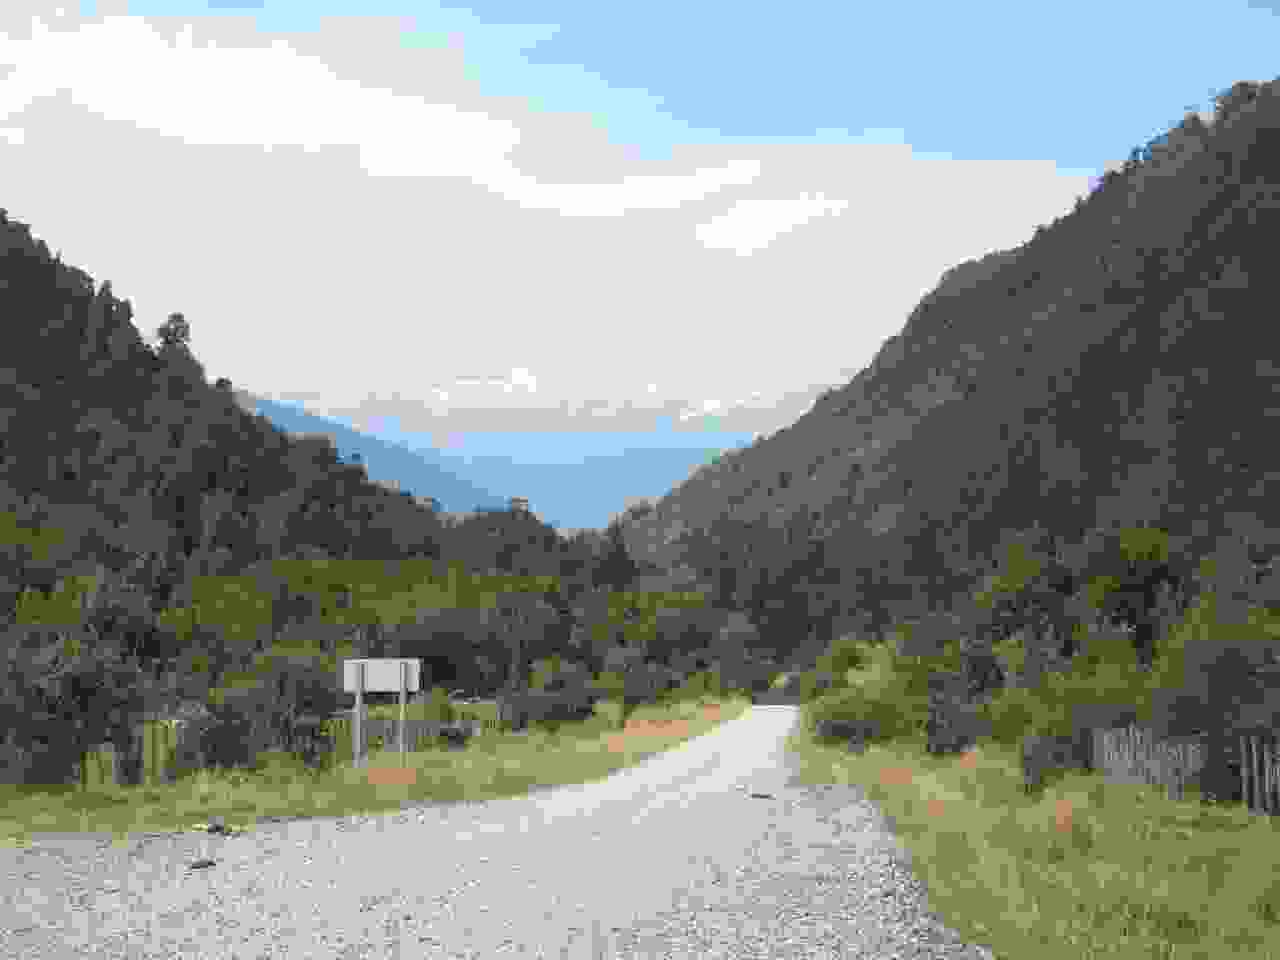
\includegraphics[height=90mm]{../wp-content/uploads/2015/02/P2202258.jpg} } 
\newline
\centerline{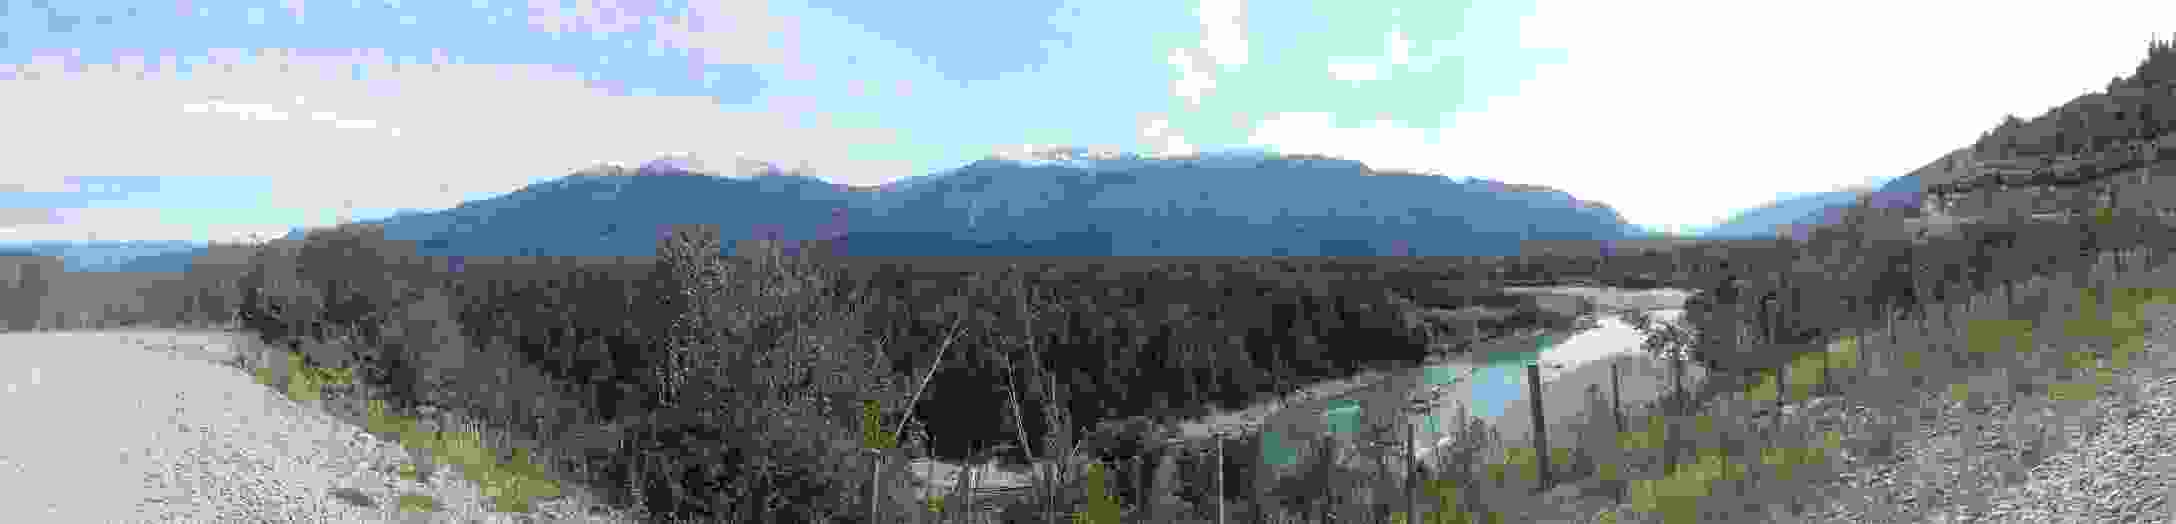
\includegraphics[height=90mm]{../wp-content/uploads/2015/02/P2202254.jpg} } 
 \newline
\centerline{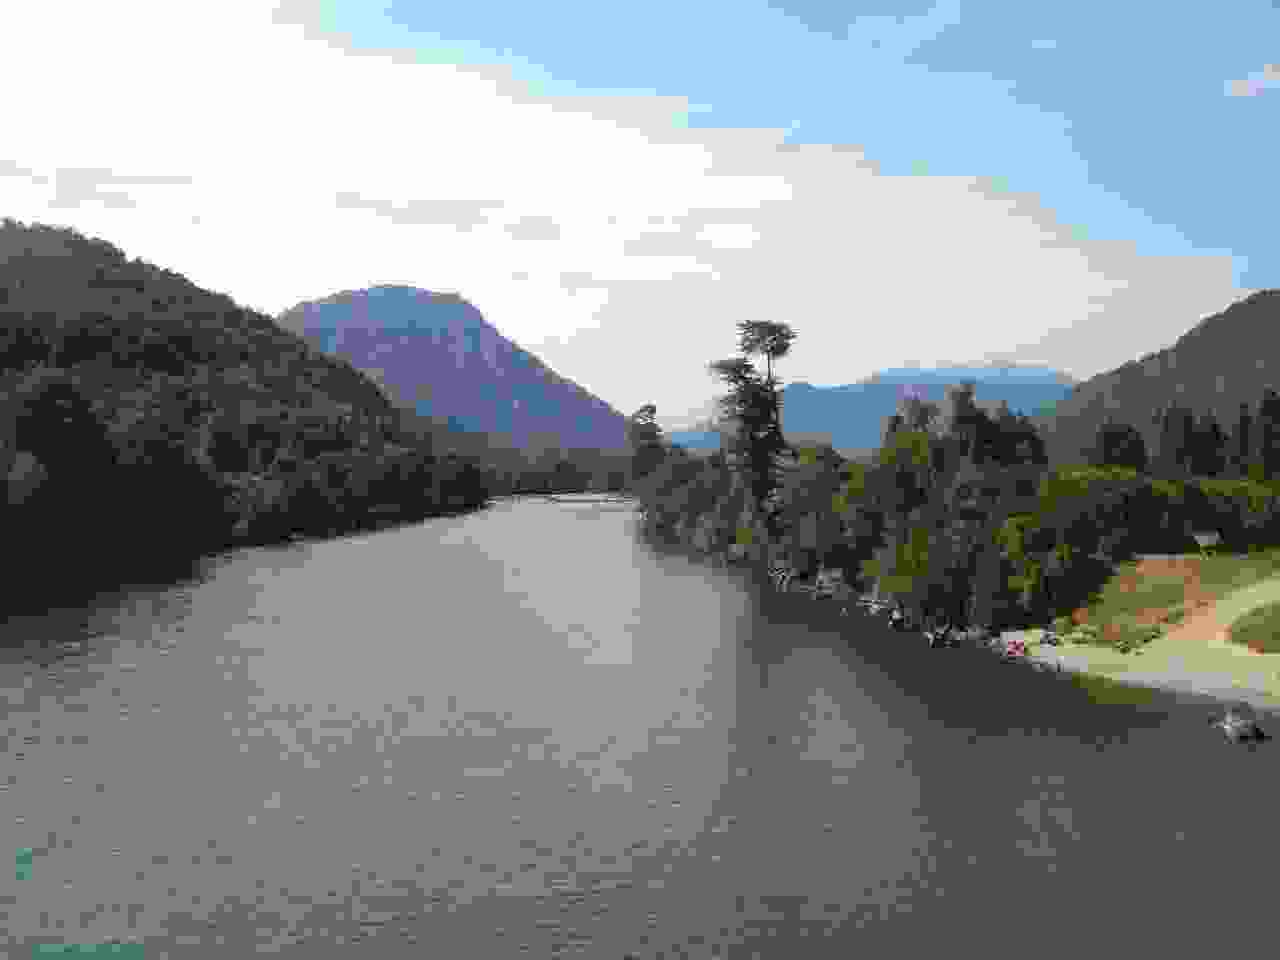
\includegraphics[height=90mm]{../wp-content/uploads/2015/02/P2202253.jpg} } 
 \newline
\centerline{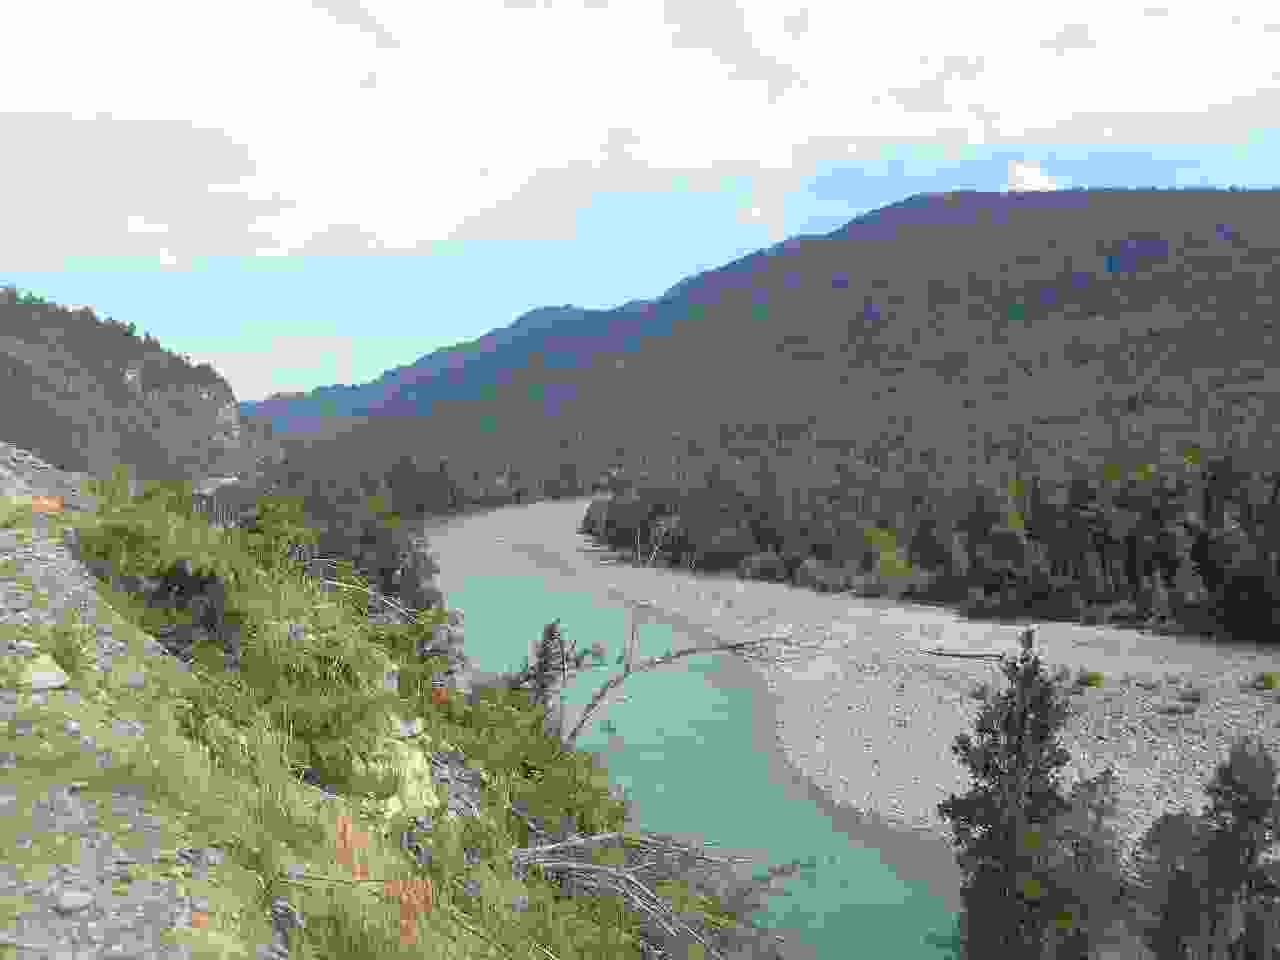
\includegraphics[height=90mm]{../wp-content/uploads/2015/02/P2202260.jpg} } 
 \newline
\centerline{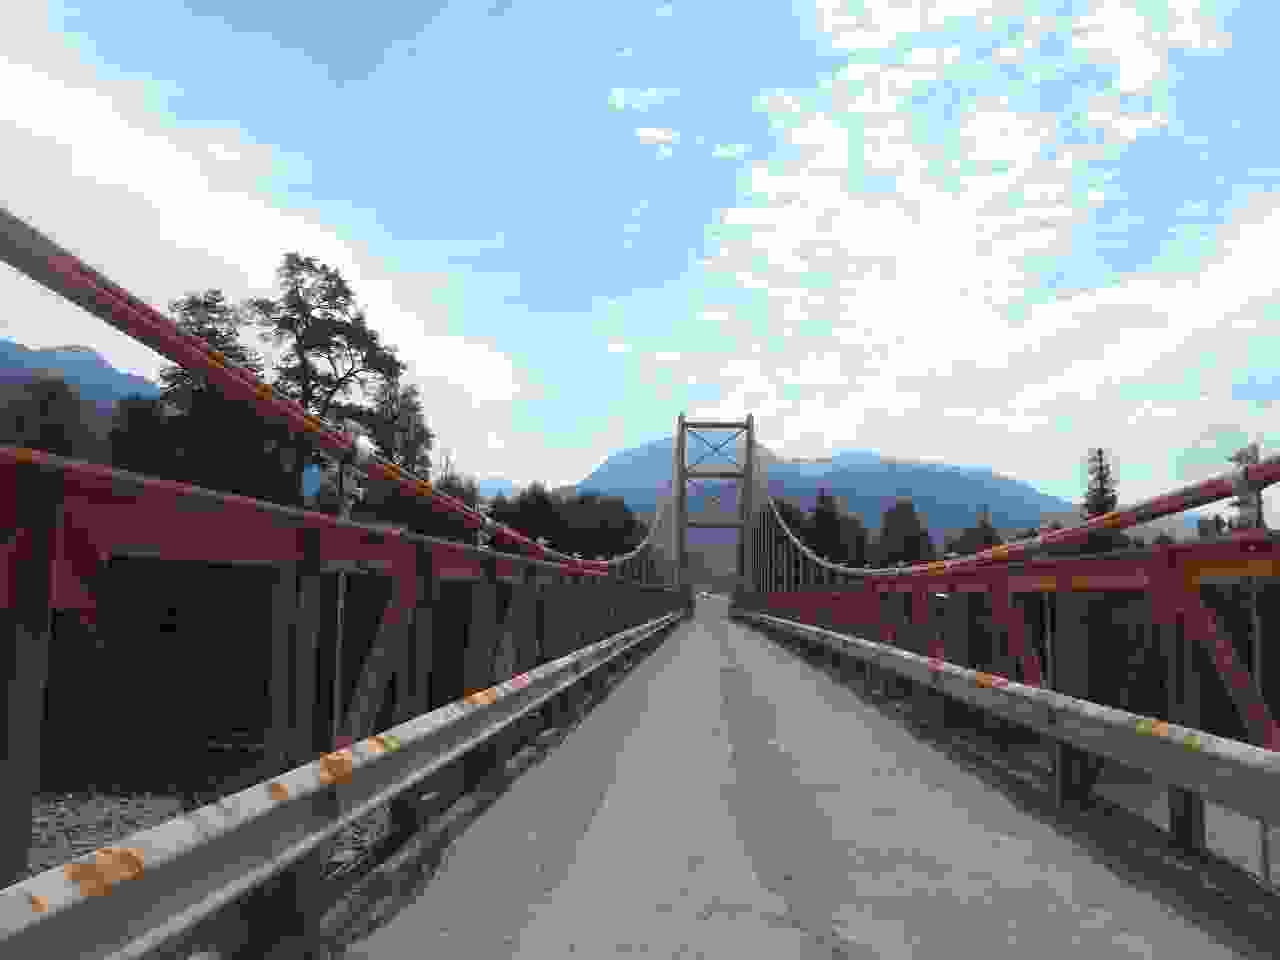
\includegraphics[height=90mm]{../wp-content/uploads/2015/02/P2202262.jpg} } 
 \newline
\centerline{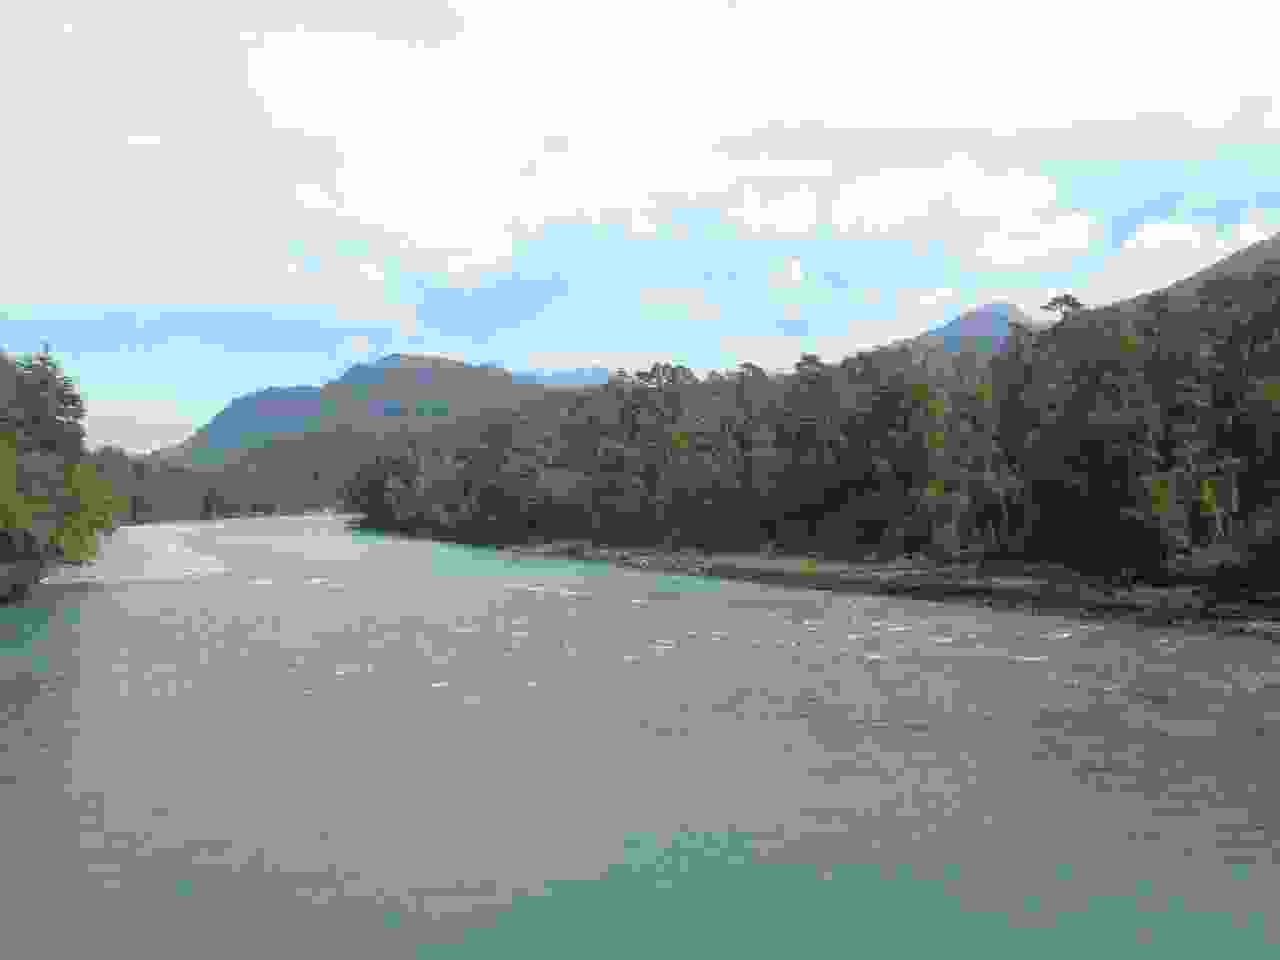
\includegraphics[height=90mm]{../wp-content/uploads/2015/02/P2202263.jpg} } 
 \newline
\centerline{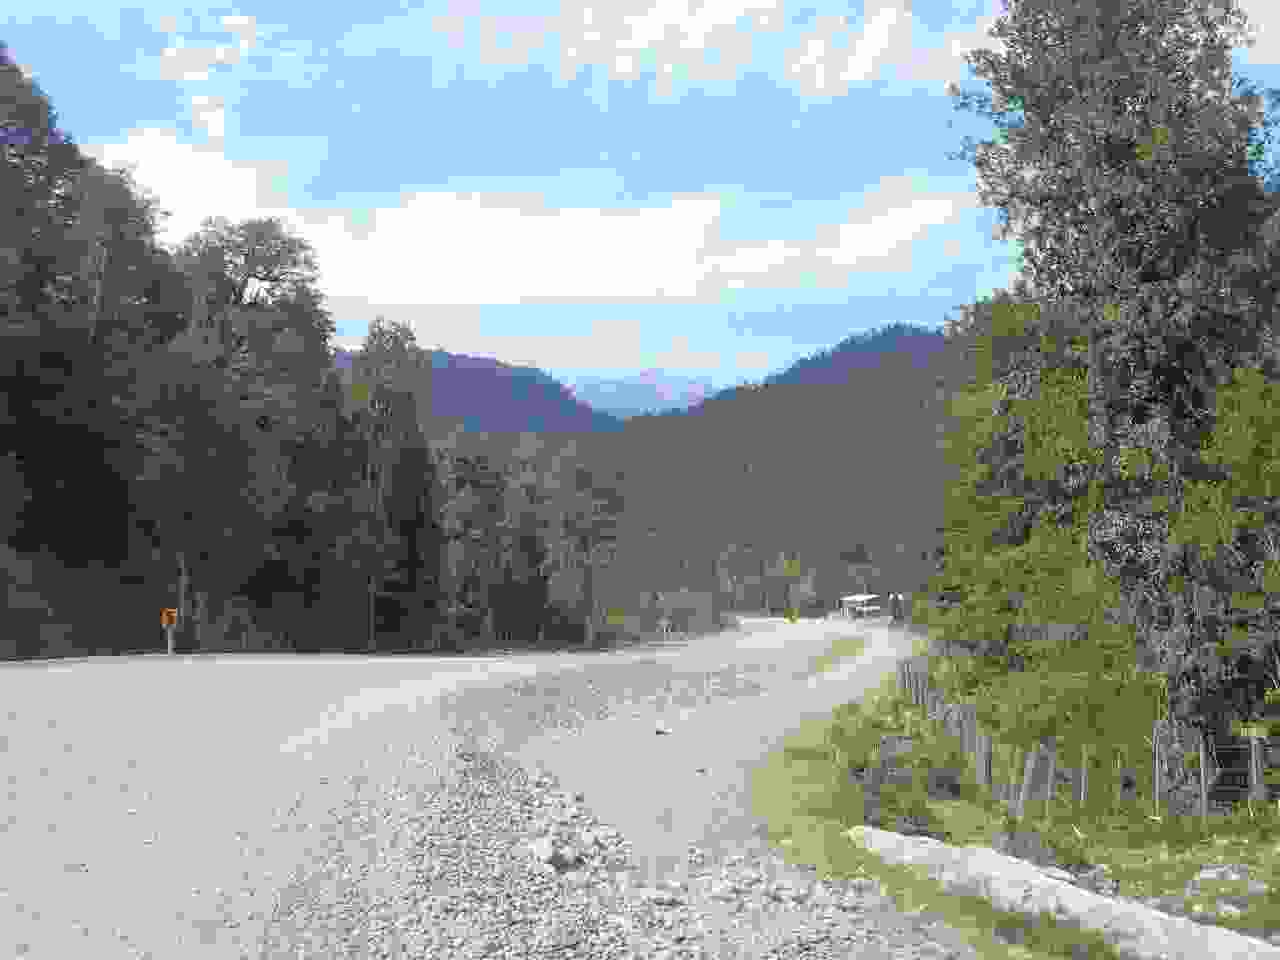
\includegraphics[height=90mm]{../wp-content/uploads/2015/02/P2202264.jpg} } 
Le passage de la piste à la route qui fait plaisir ! \newline
 \newline
\centerline{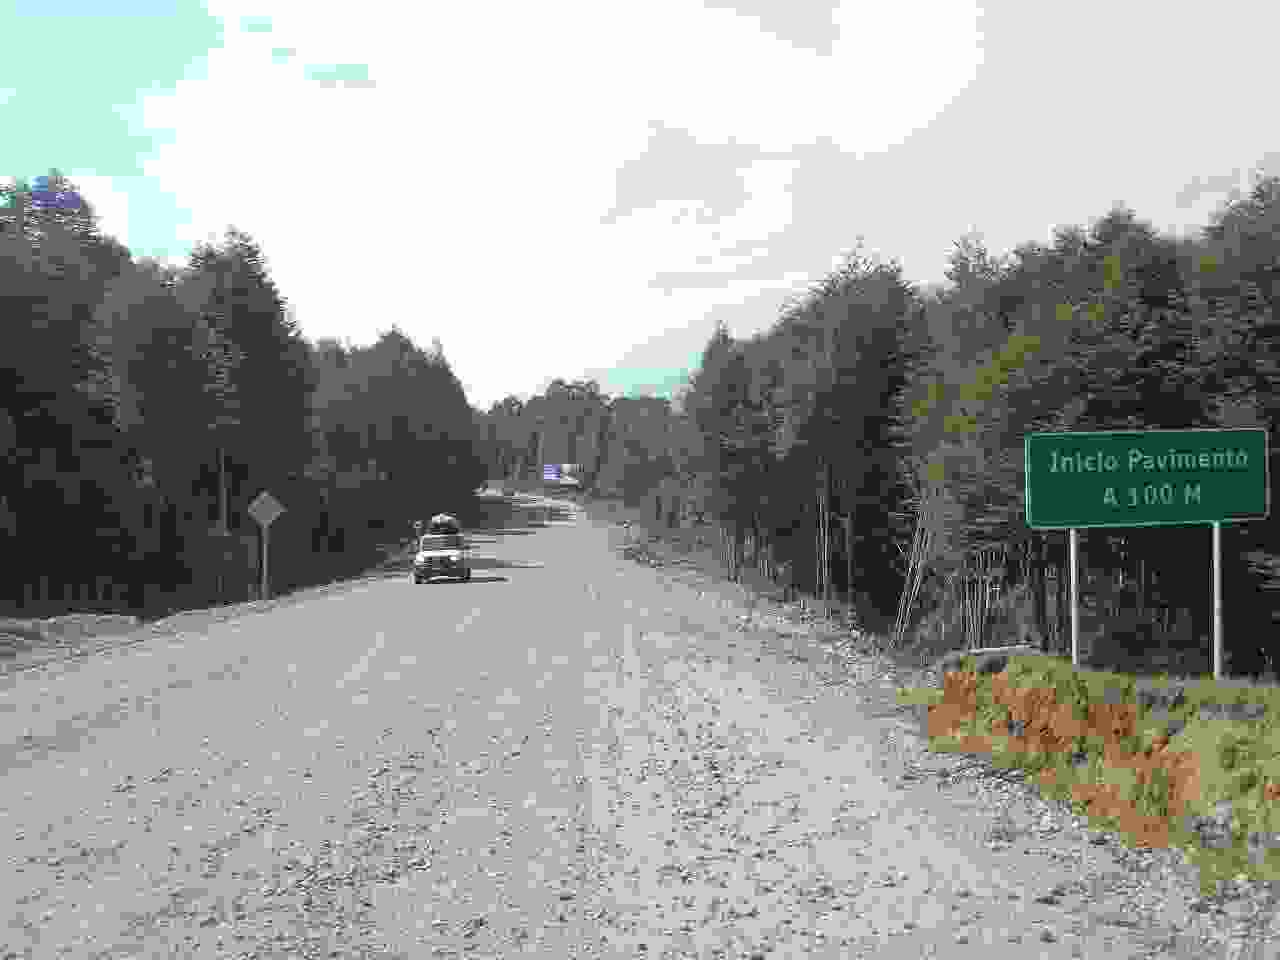
\includegraphics[height=90mm]{../wp-content/uploads/2015/02/P2202265.jpg} } 
\newline
\centerline{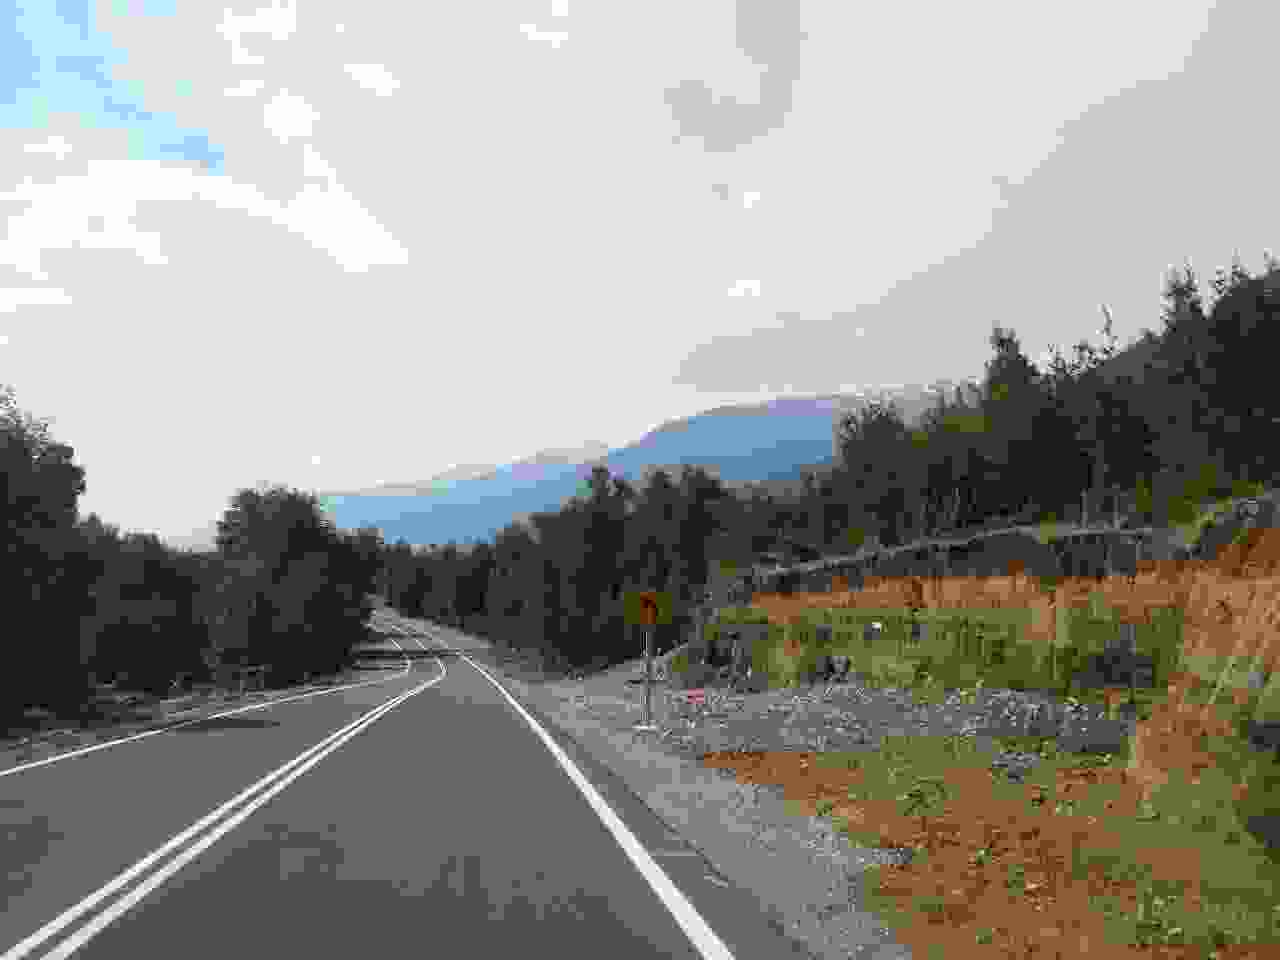
\includegraphics[height=90mm]{../wp-content/uploads/2015/02/P2202266.jpg} } 
 \newline
\centerline{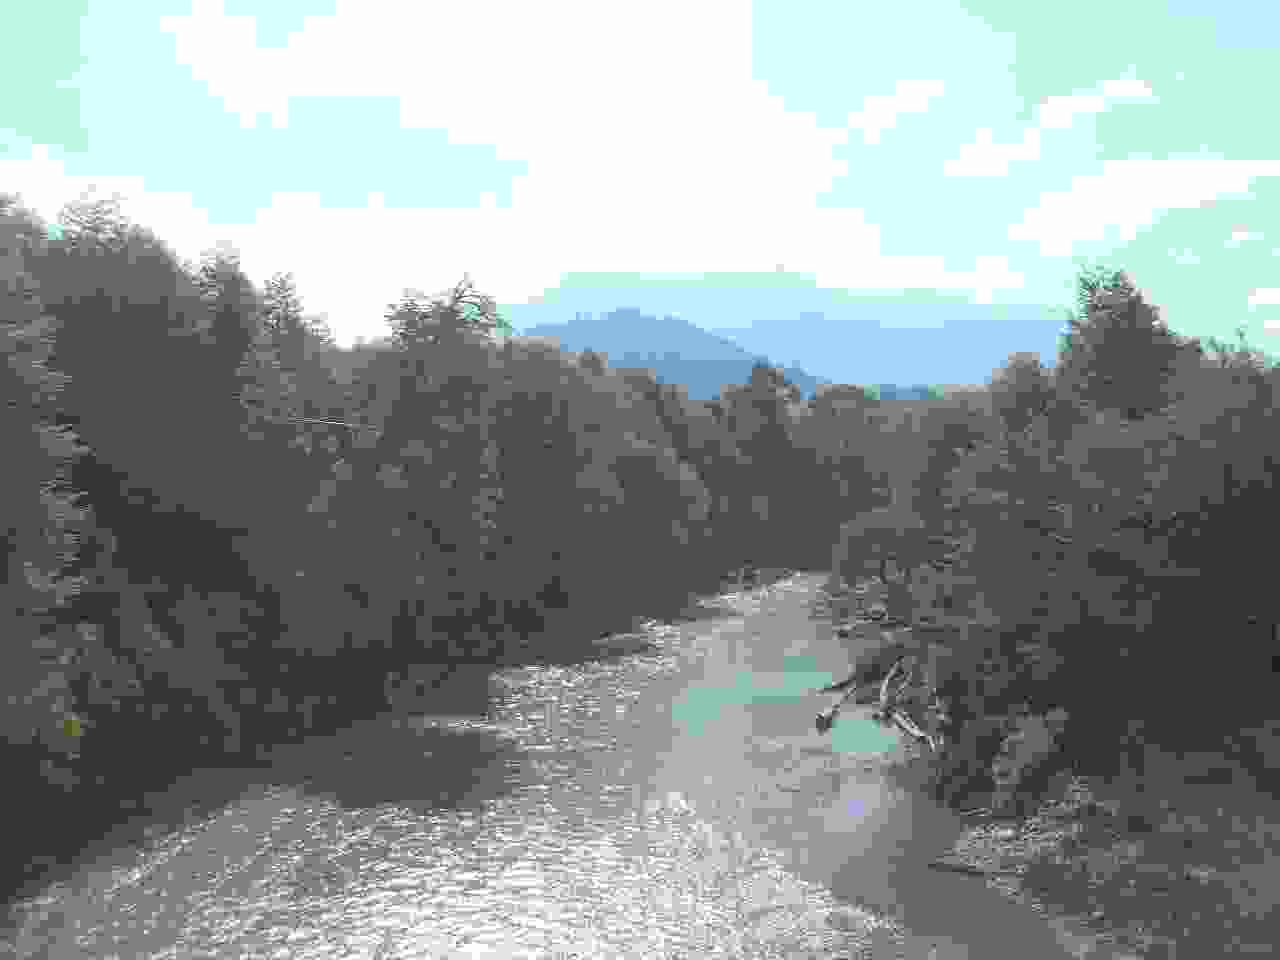
\includegraphics[height=90mm]{../wp-content/uploads/2015/02/P2202267.jpg} } 
 \newline
\centerline{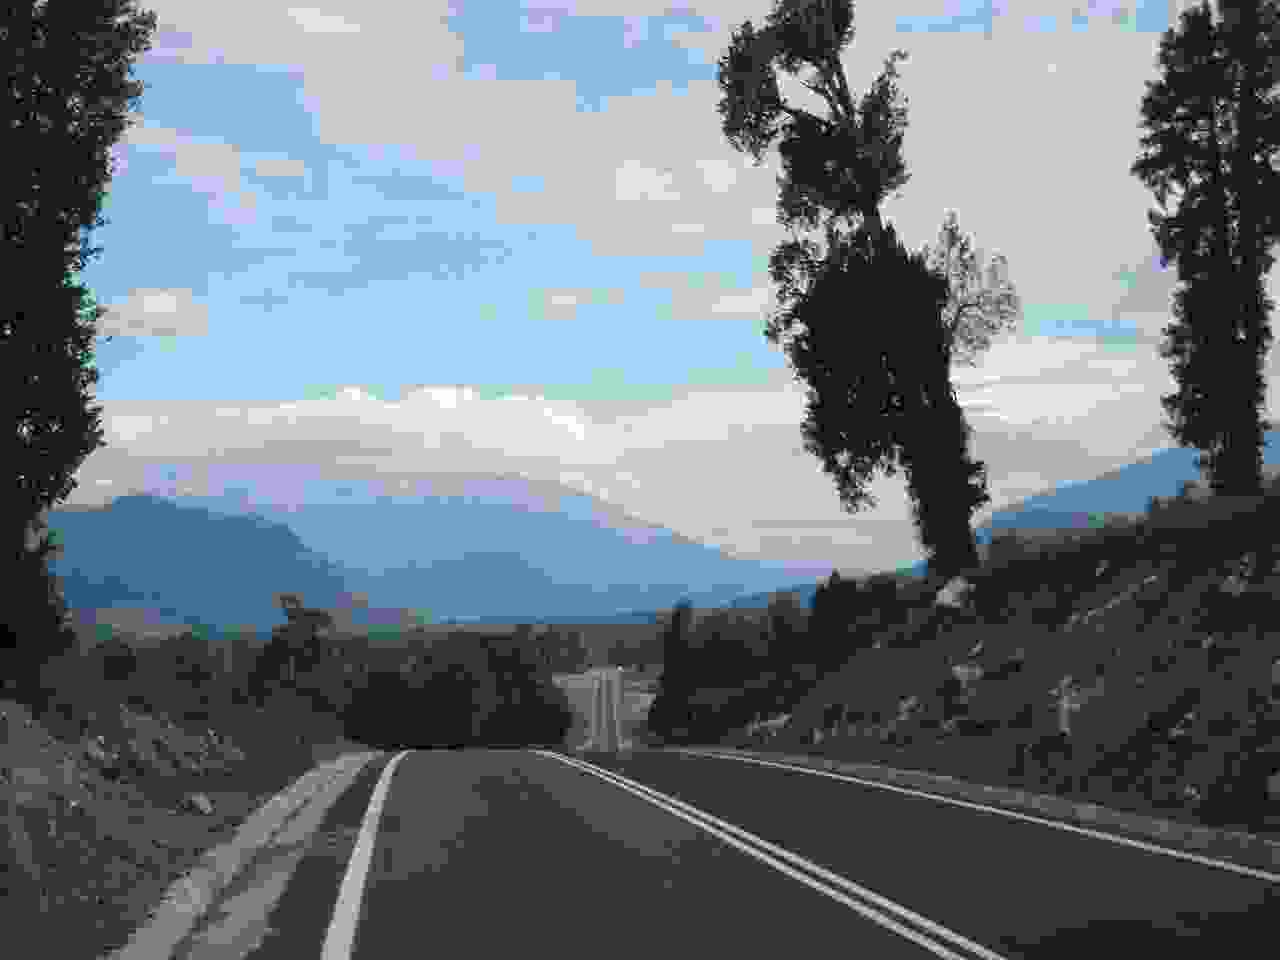
\includegraphics[height=90mm]{../wp-content/uploads/2015/02/P2202269.jpg} } 
Pas mal d`autres voyageurs à velo dans les campings \newline
 \newline
\centerline{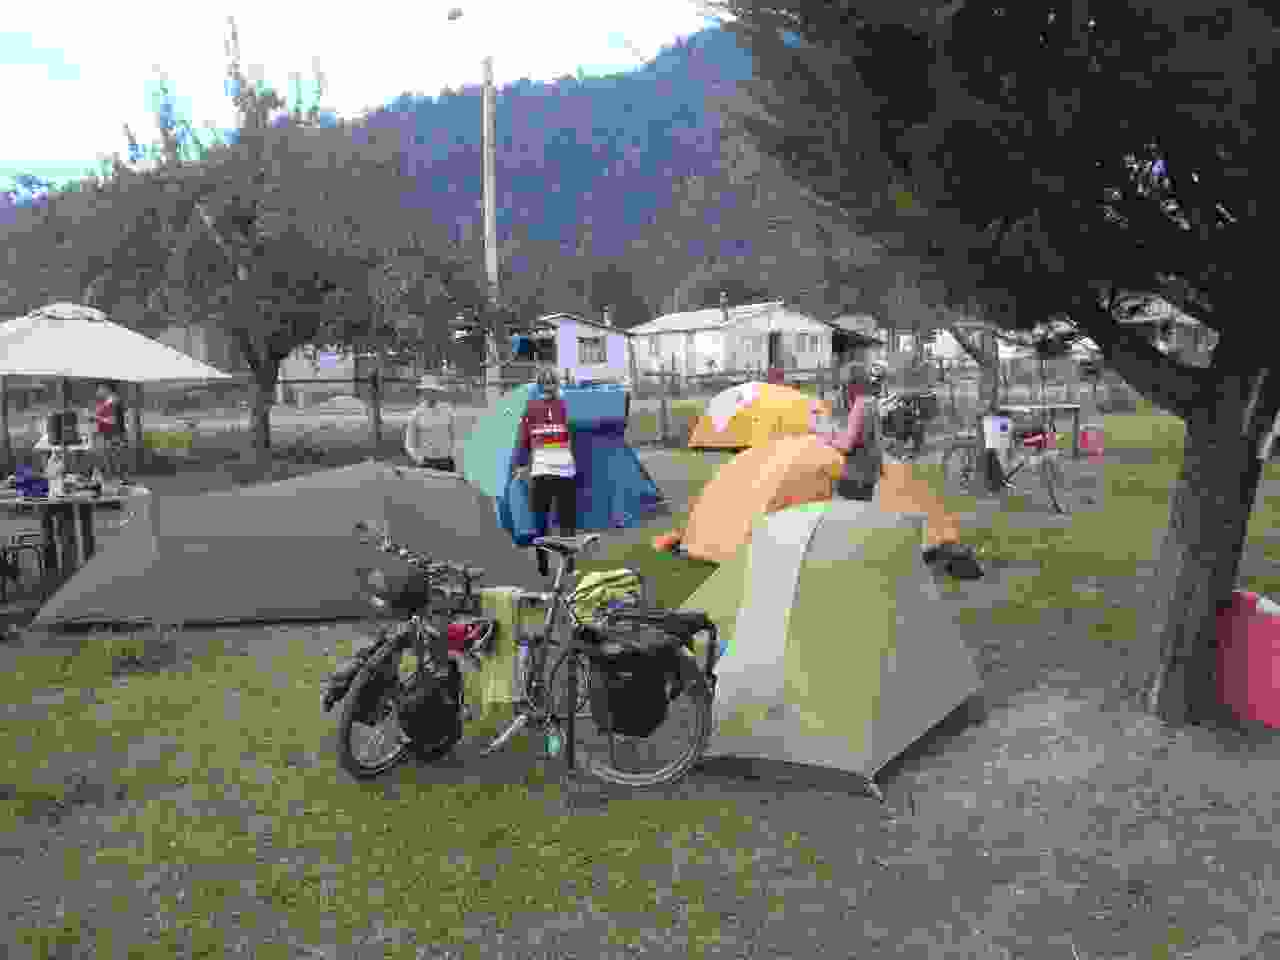
\includegraphics[height=90mm]{../wp-content/uploads/2015/02/P2212275.jpg} } 
Deuxième étape jusqu'à Chaiten. \newline
 \newline
\centerline{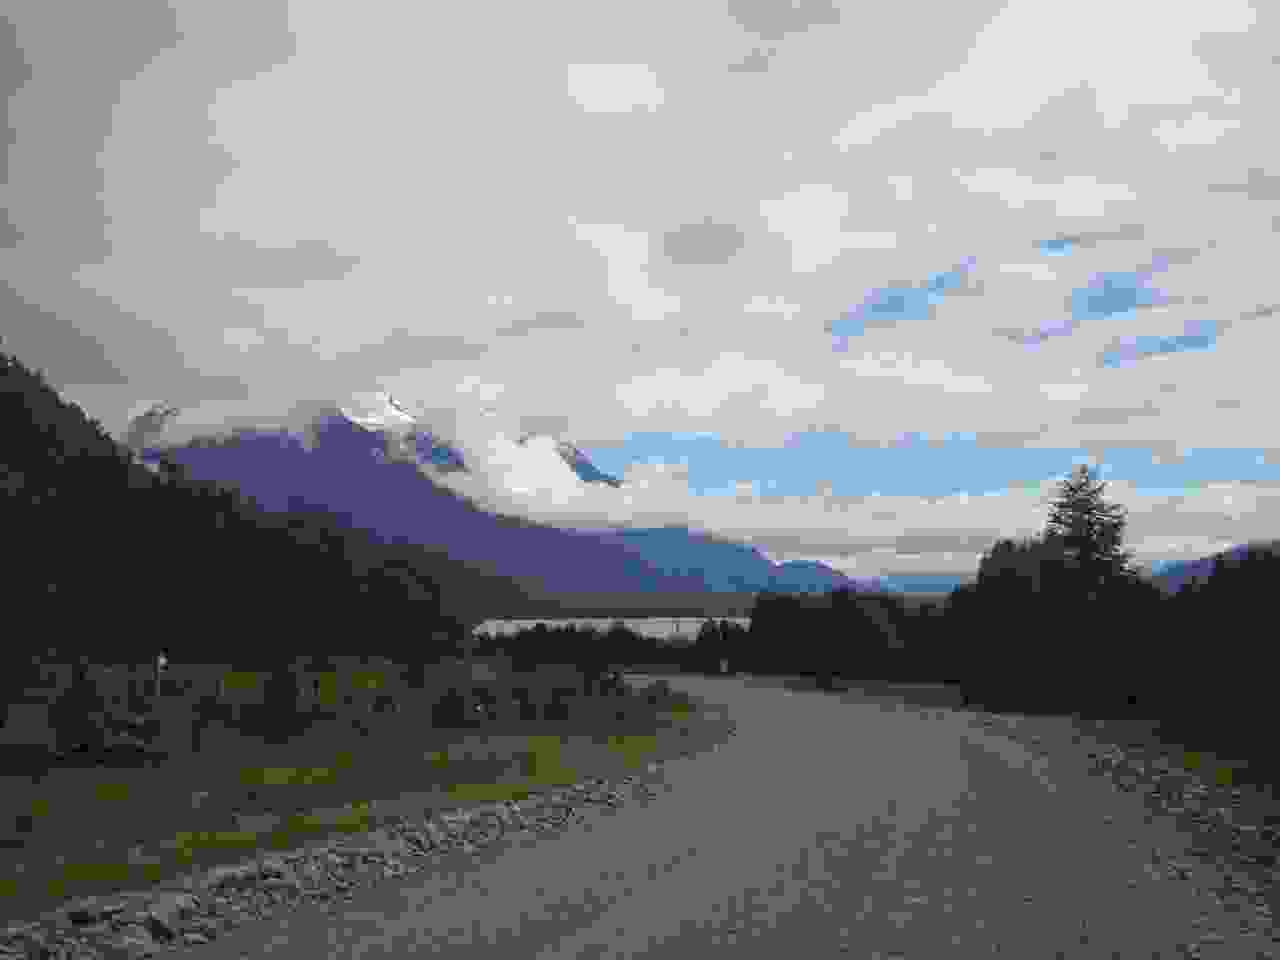
\includegraphics[height=90mm]{../wp-content/uploads/2015/02/P2212277.jpg} } 
 \newline
\centerline{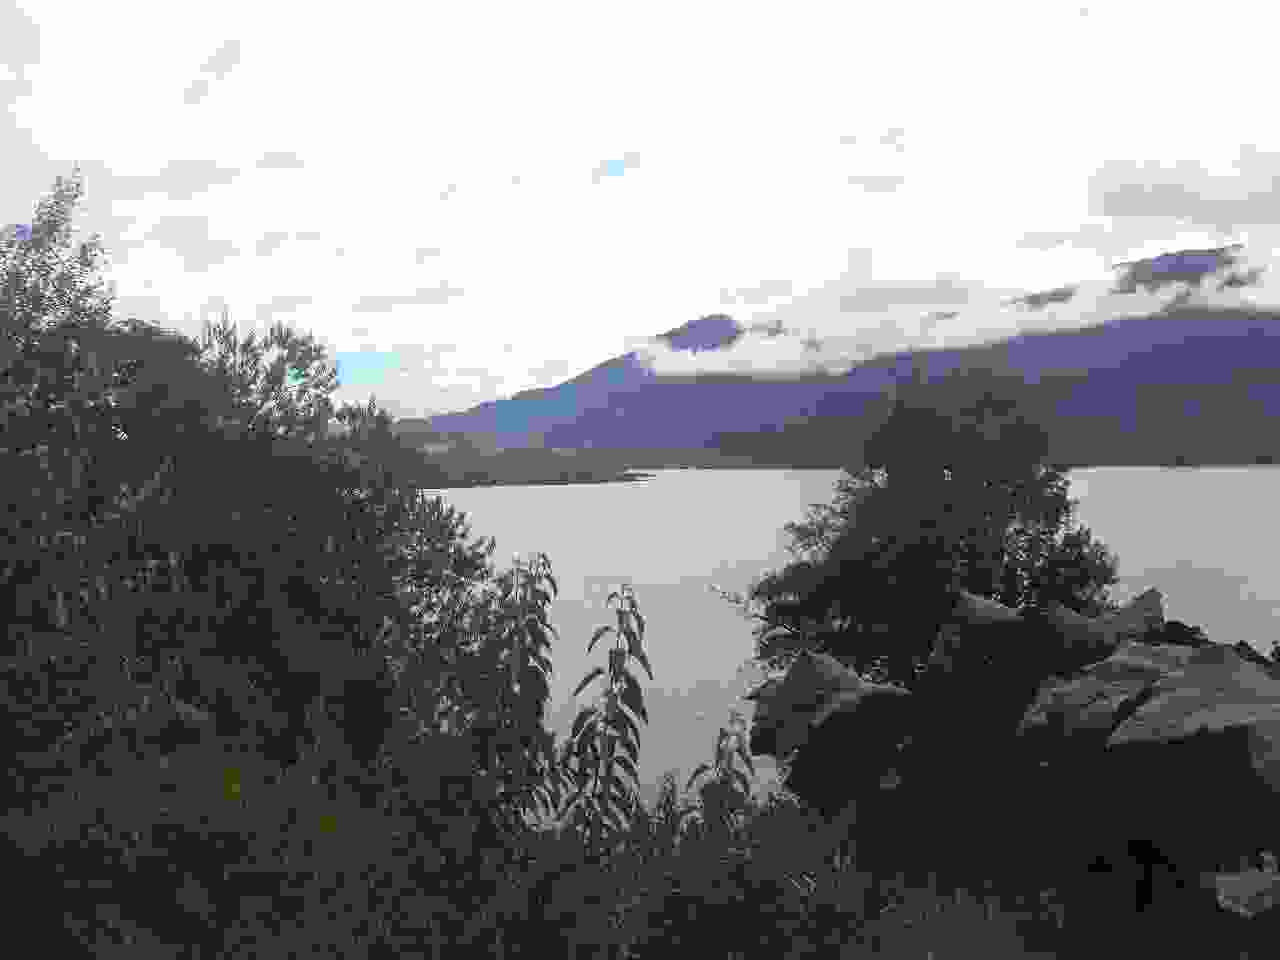
\includegraphics[height=90mm]{../wp-content/uploads/2015/02/P2212280.jpg} } 
 \newline
\centerline{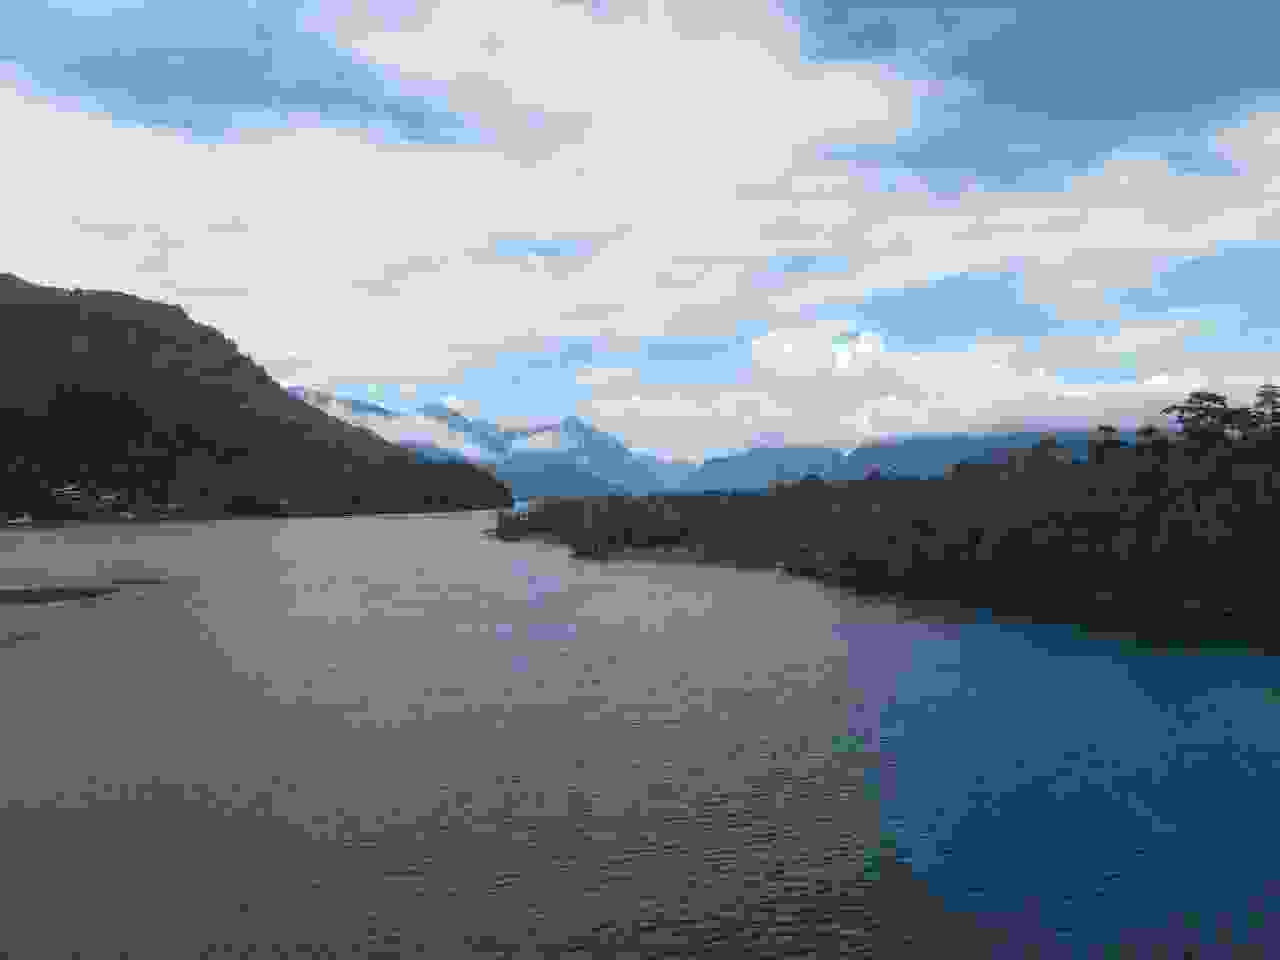
\includegraphics[height=90mm]{../wp-content/uploads/2015/02/P2212281.jpg} } 
 \newline
\centerline{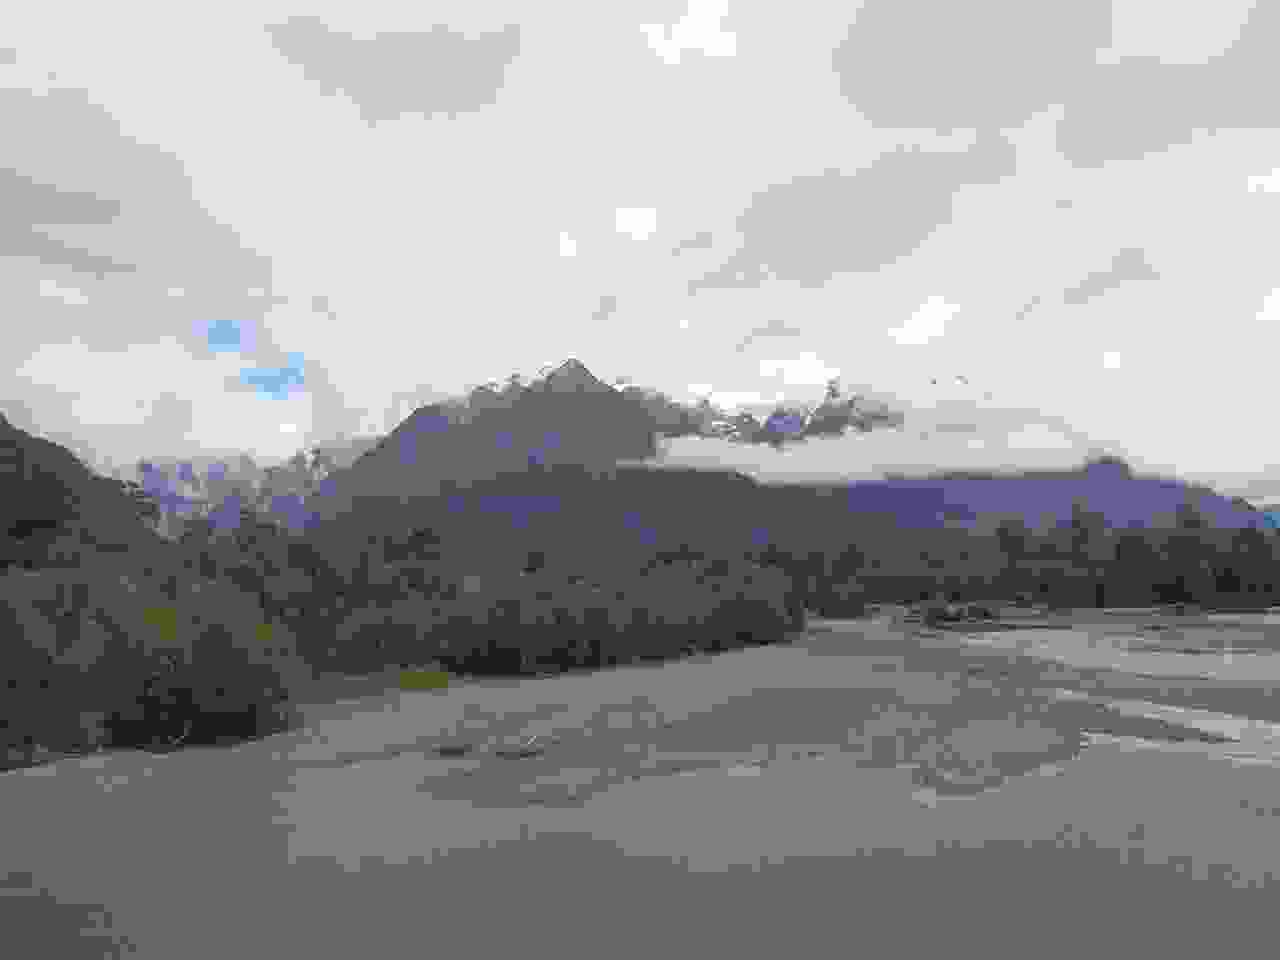
\includegraphics[height=90mm]{../wp-content/uploads/2015/02/P2212283.jpg} } 
 \newline
\centerline{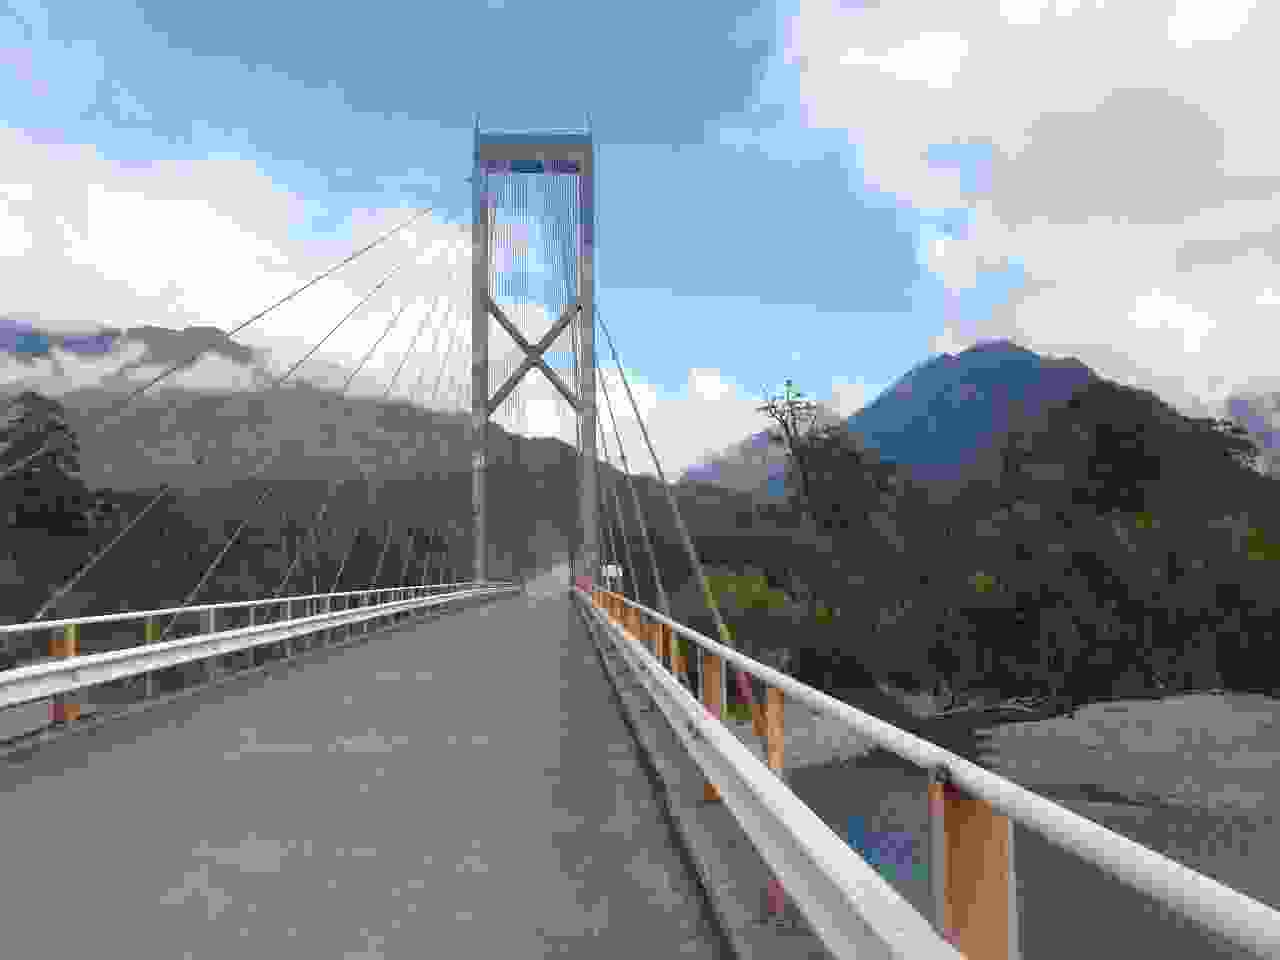
\includegraphics[height=90mm]{../wp-content/uploads/2015/02/P2212284.jpg} } 
 \newline
\centerline{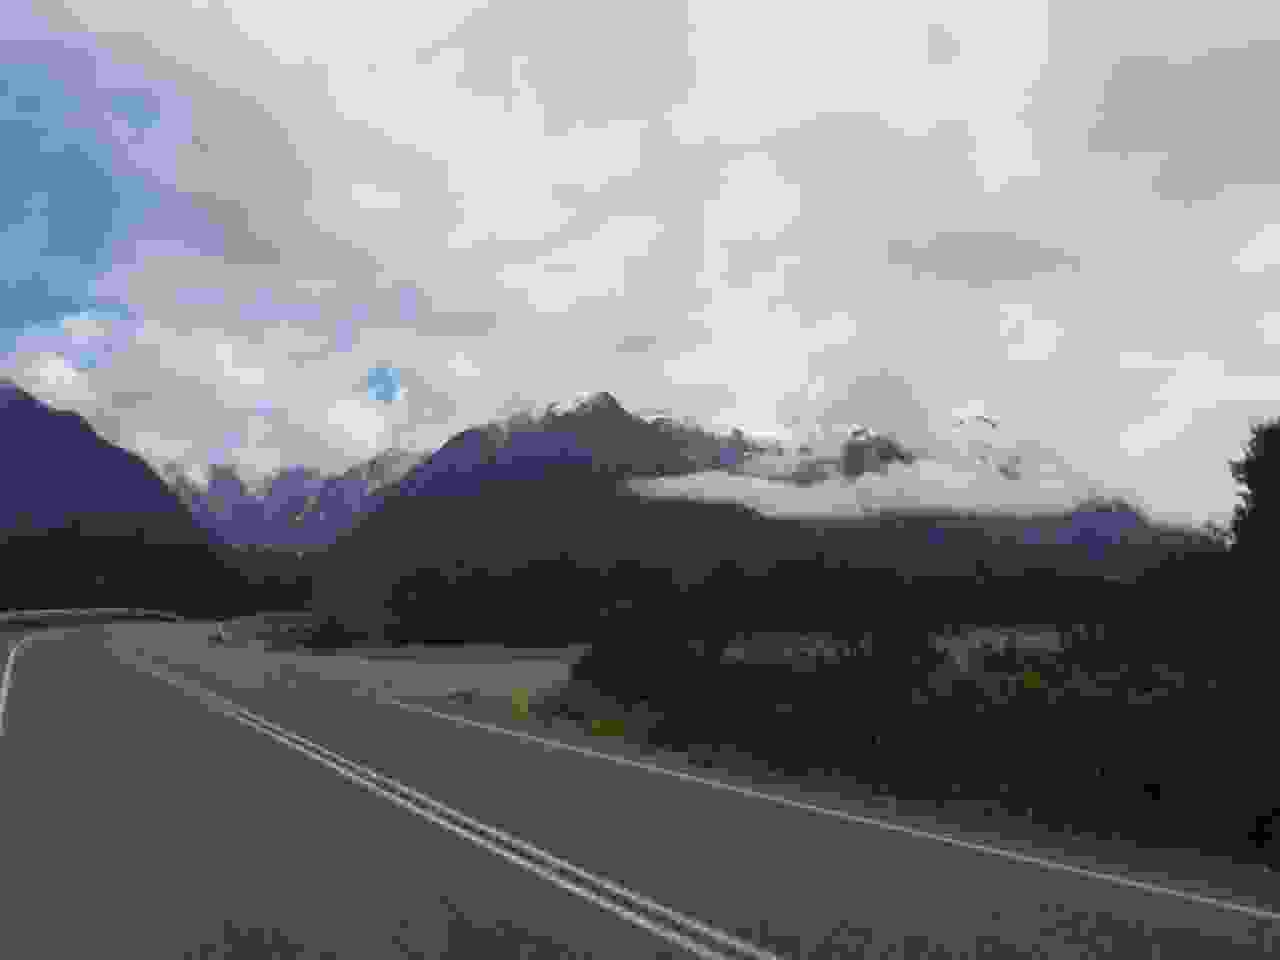
\includegraphics[height=90mm]{../wp-content/uploads/2015/02/P2212285.jpg} } 
 \newline
\centerline{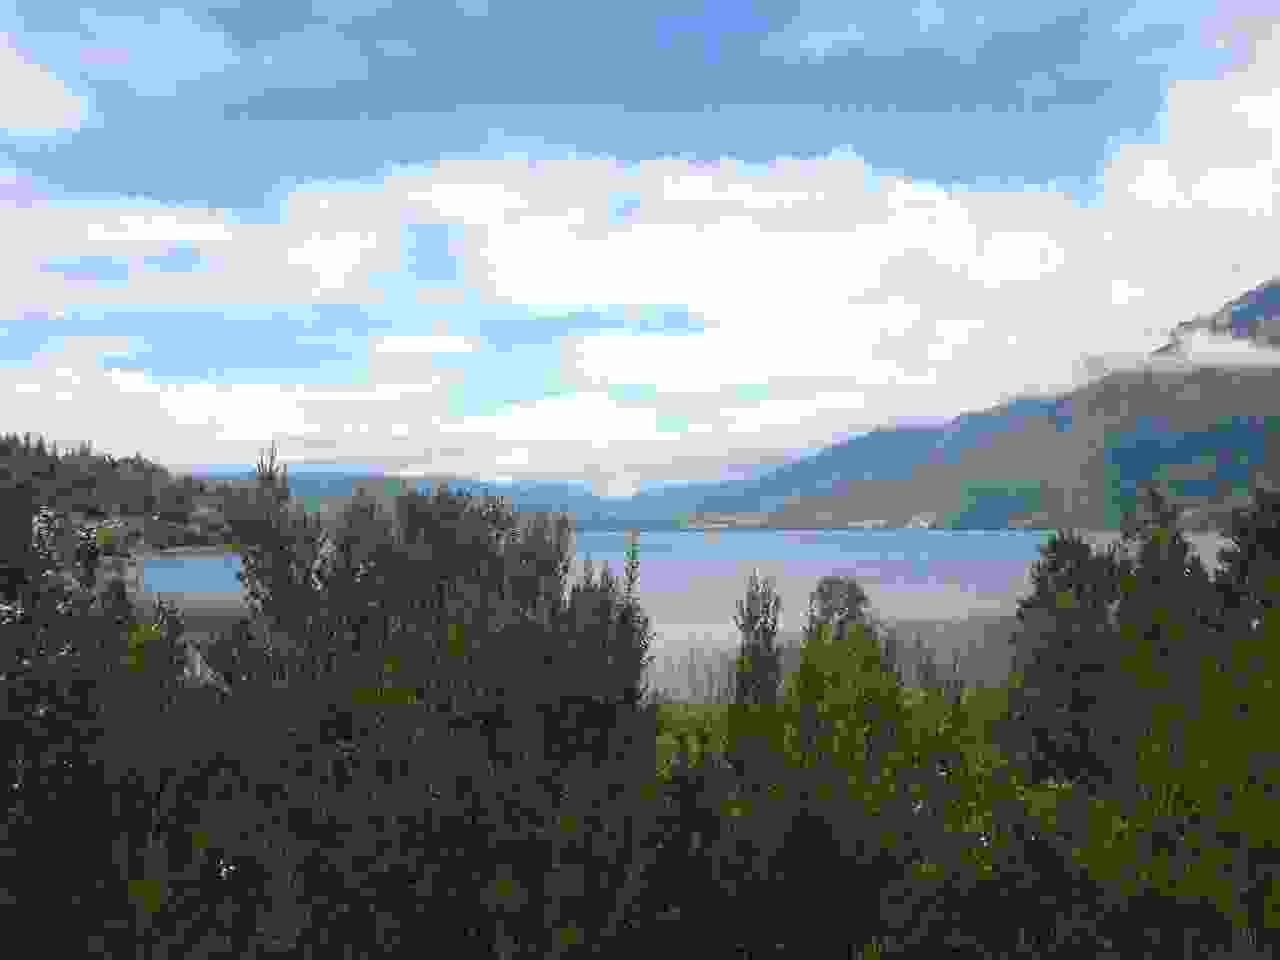
\includegraphics[height=90mm]{../wp-content/uploads/2015/02/P2212286.jpg} } 
 \newline
\centerline{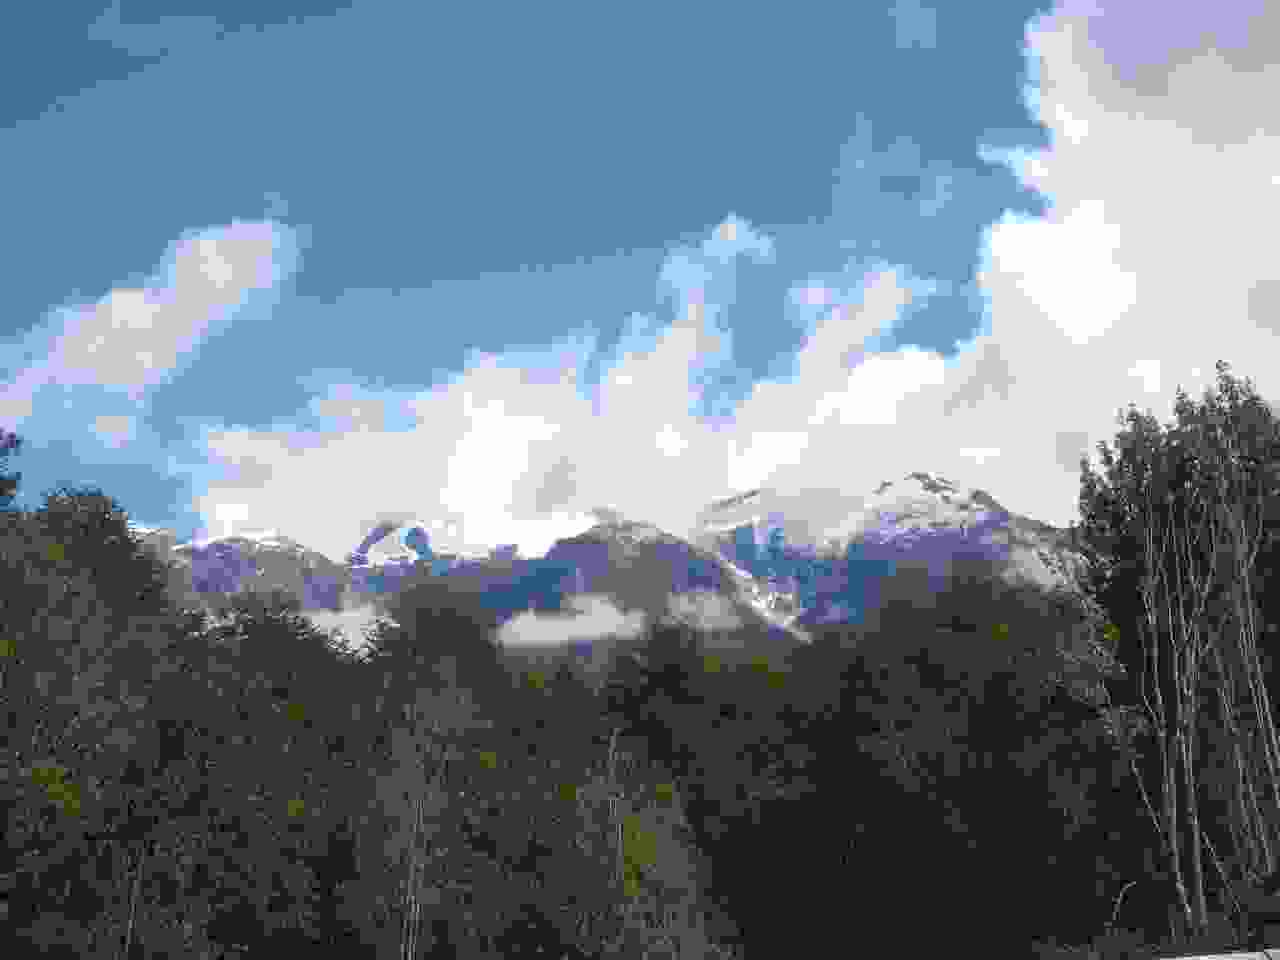
\includegraphics[height=90mm]{../wp-content/uploads/2015/02/P2212288.jpg} } 
 \newline
\centerline{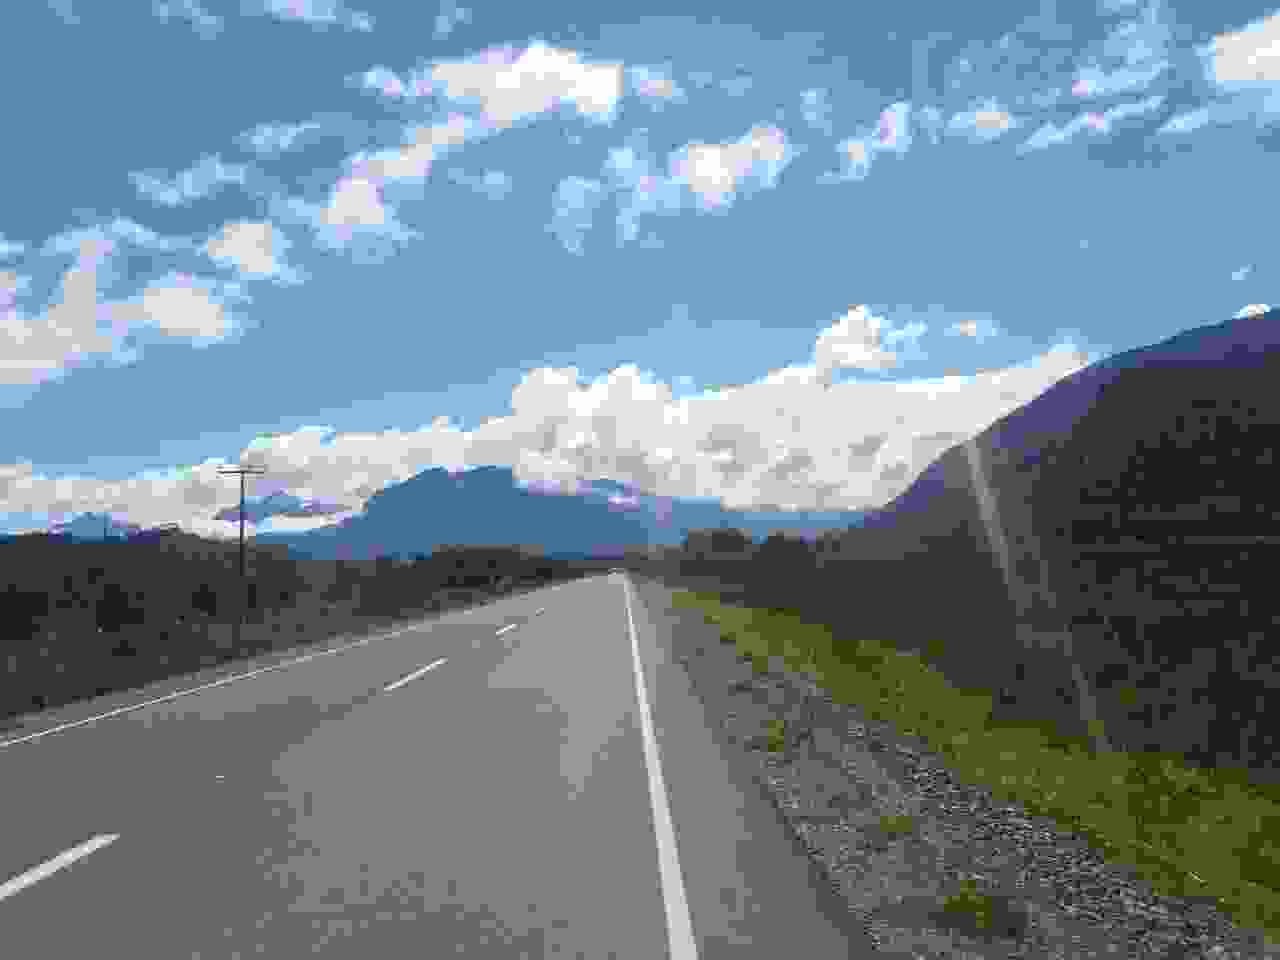
\includegraphics[height=90mm]{../wp-content/uploads/2015/02/P2212290.jpg} } 
Petit détour pour profiter des thermes d'eau chaude. \newline
 \newline
\centerline{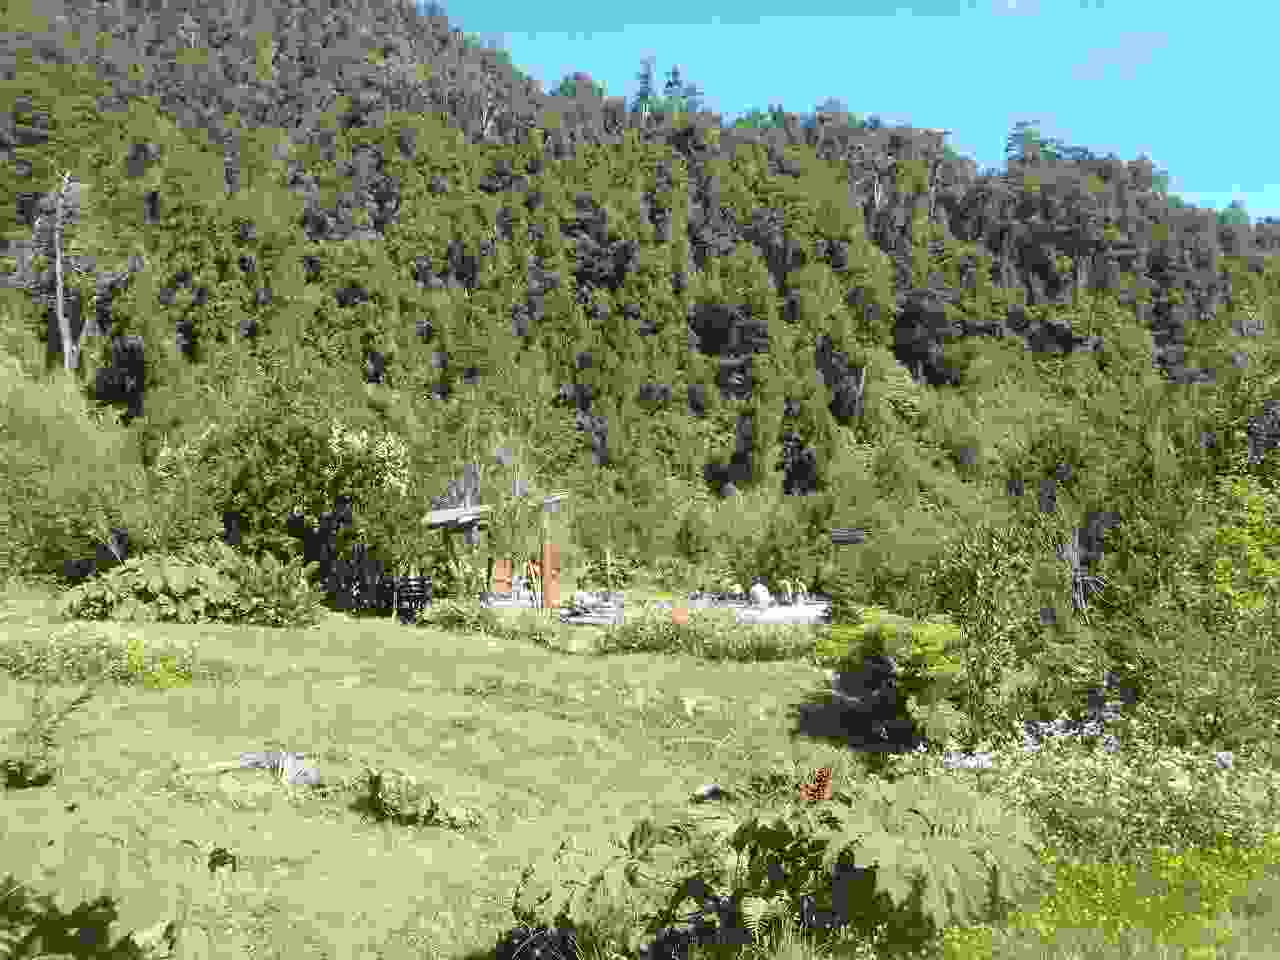
\includegraphics[height=90mm]{../wp-content/uploads/2015/02/P2212292.jpg} } 
\newline
\centerline{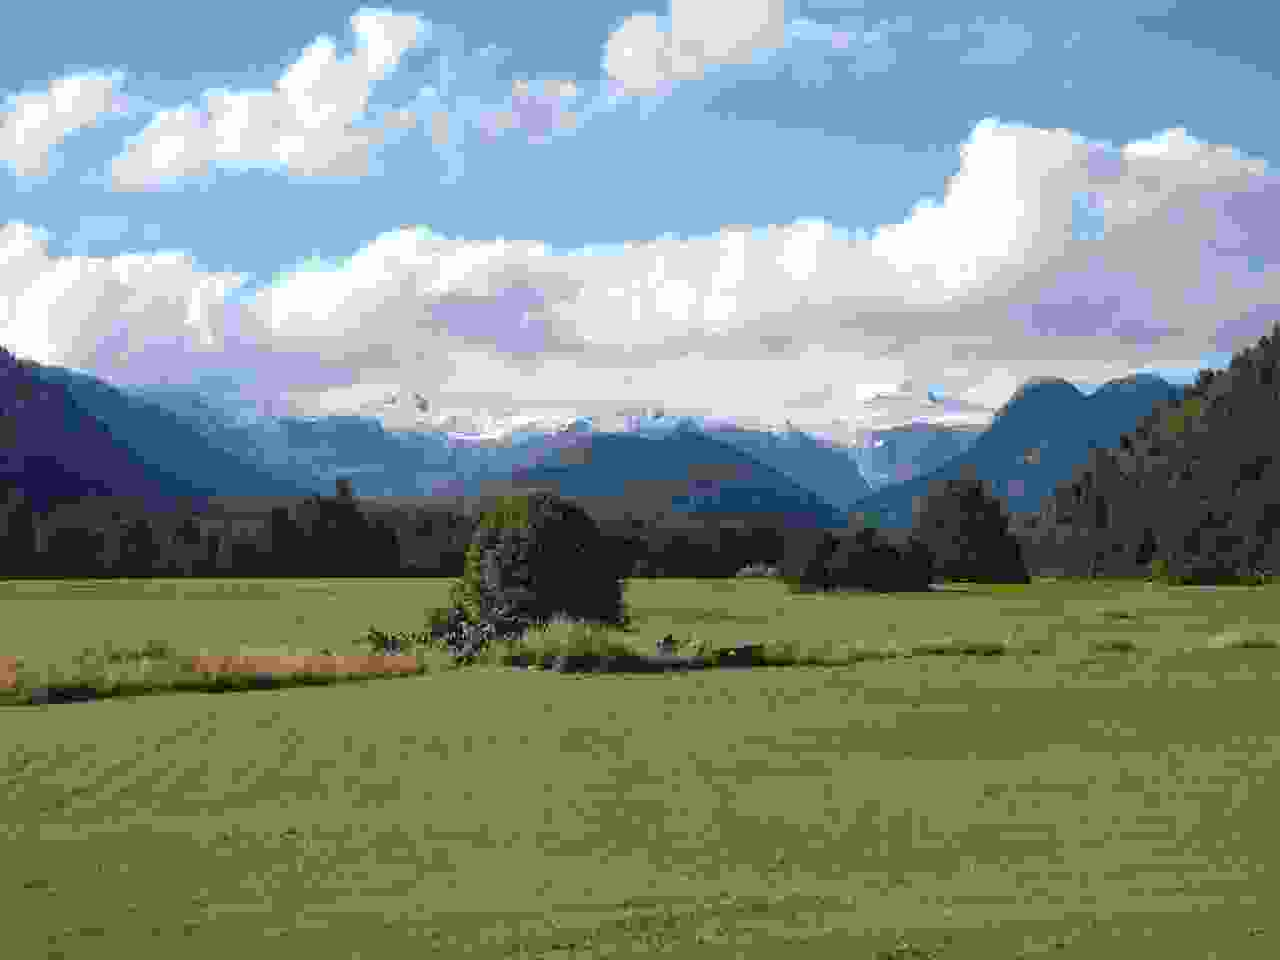
\includegraphics[height=90mm]{../wp-content/uploads/2015/02/P2212294.jpg} } 
 \newline
\centerline{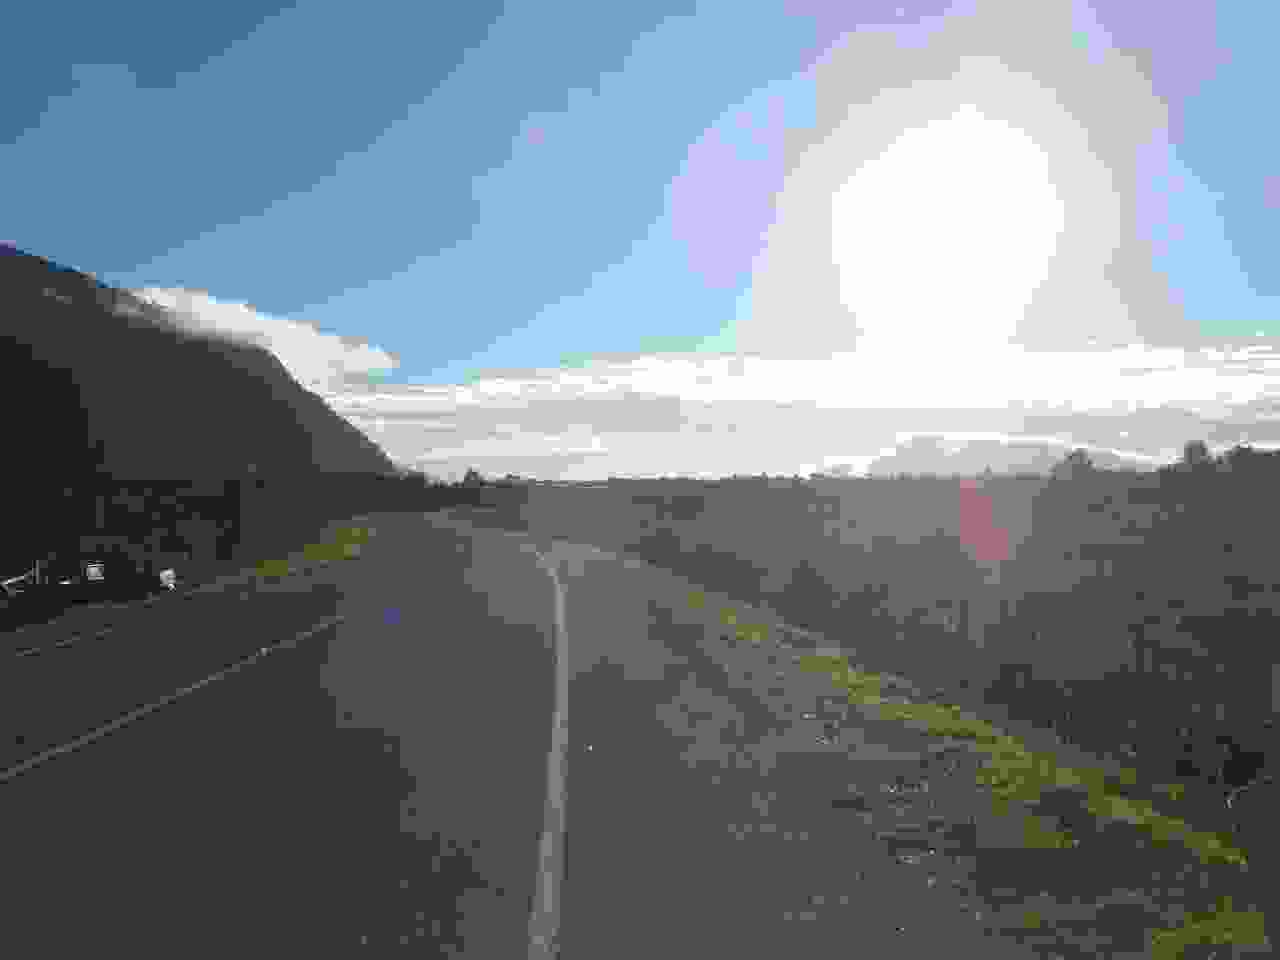
\includegraphics[height=90mm]{../wp-content/uploads/2015/02/P2222297.jpg} } 
A Chaiten, je suis invité par une famille chilienne rencontrée à une fête locale sur la route. \newline
 \newline
\centerline{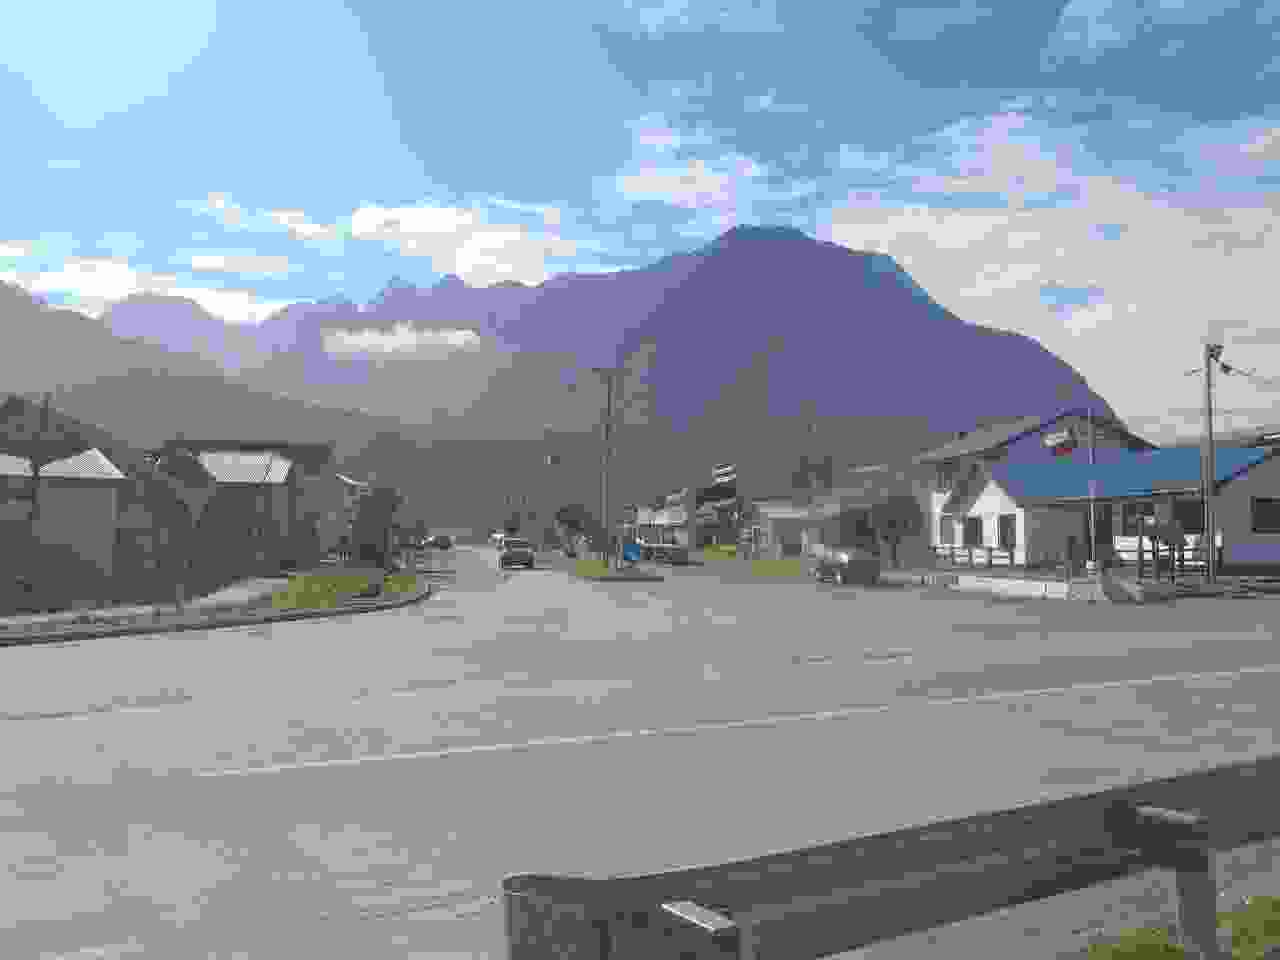
\includegraphics[height=90mm]{../wp-content/uploads/2015/02/P2232319.jpg} } 
 \newline
\centerline{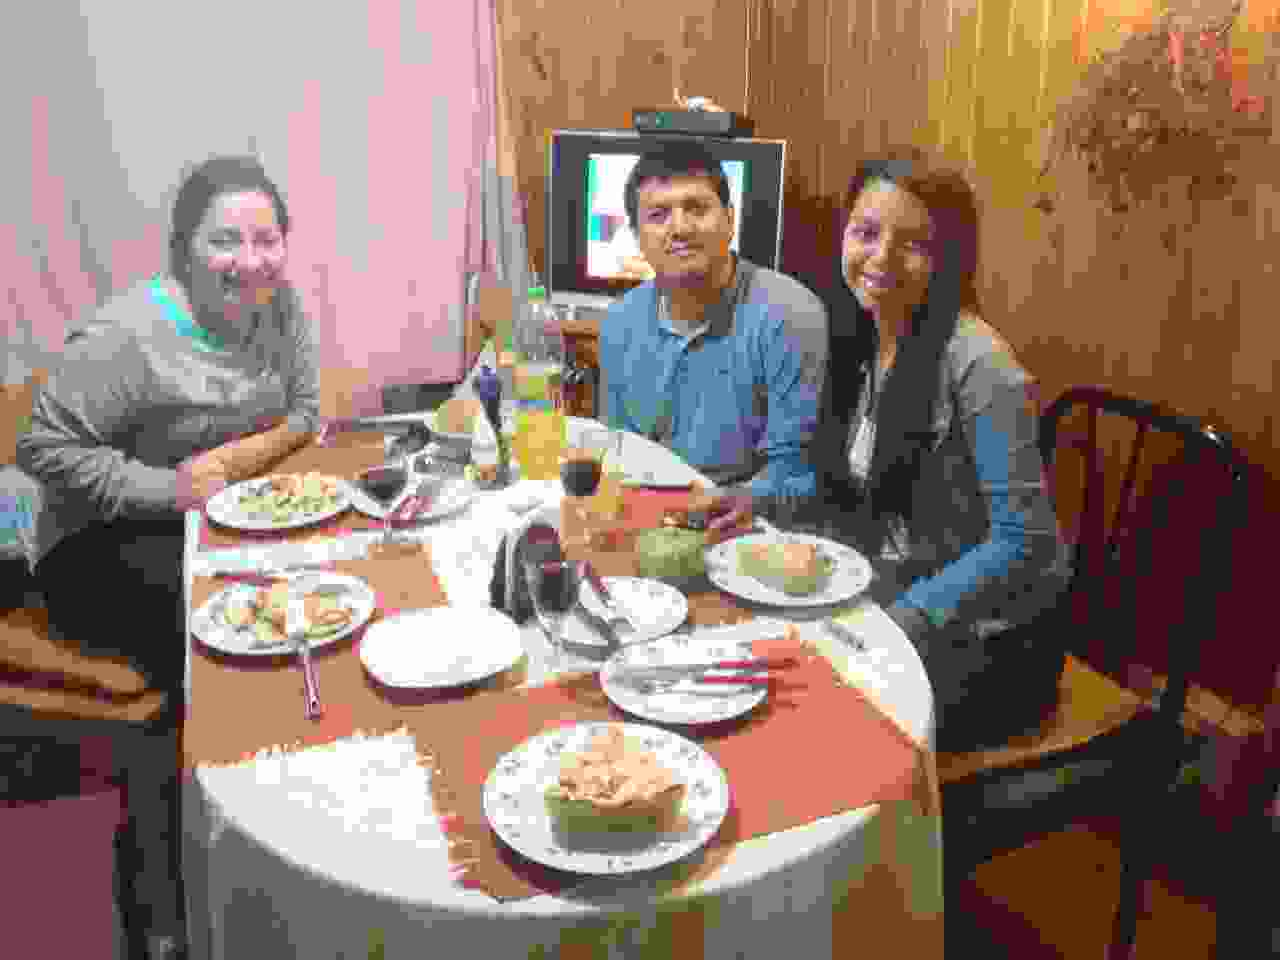
\includegraphics[height=90mm]{../wp-content/uploads/2015/02/P2232314.jpg} } 
 \newline
\centerline{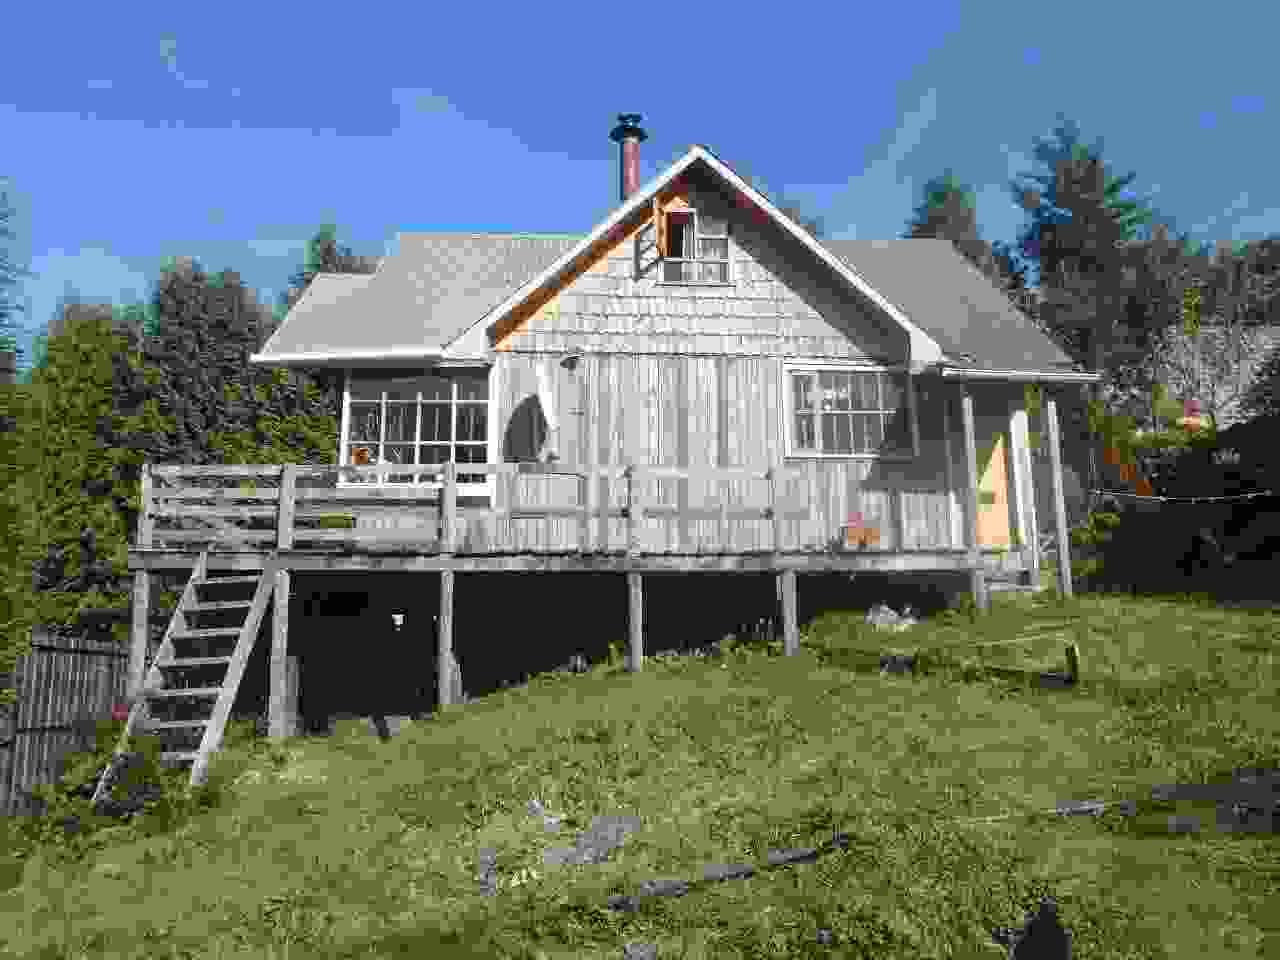
\includegraphics[height=90mm]{../wp-content/uploads/2015/02/P2232317.jpg} } 
Du coup, je reste 2 jours ce qui me permet de faire l'ascension du volcan Chaiten, 962m de haut et entré en éruption en 2008. \newline
 \newline
\centerline{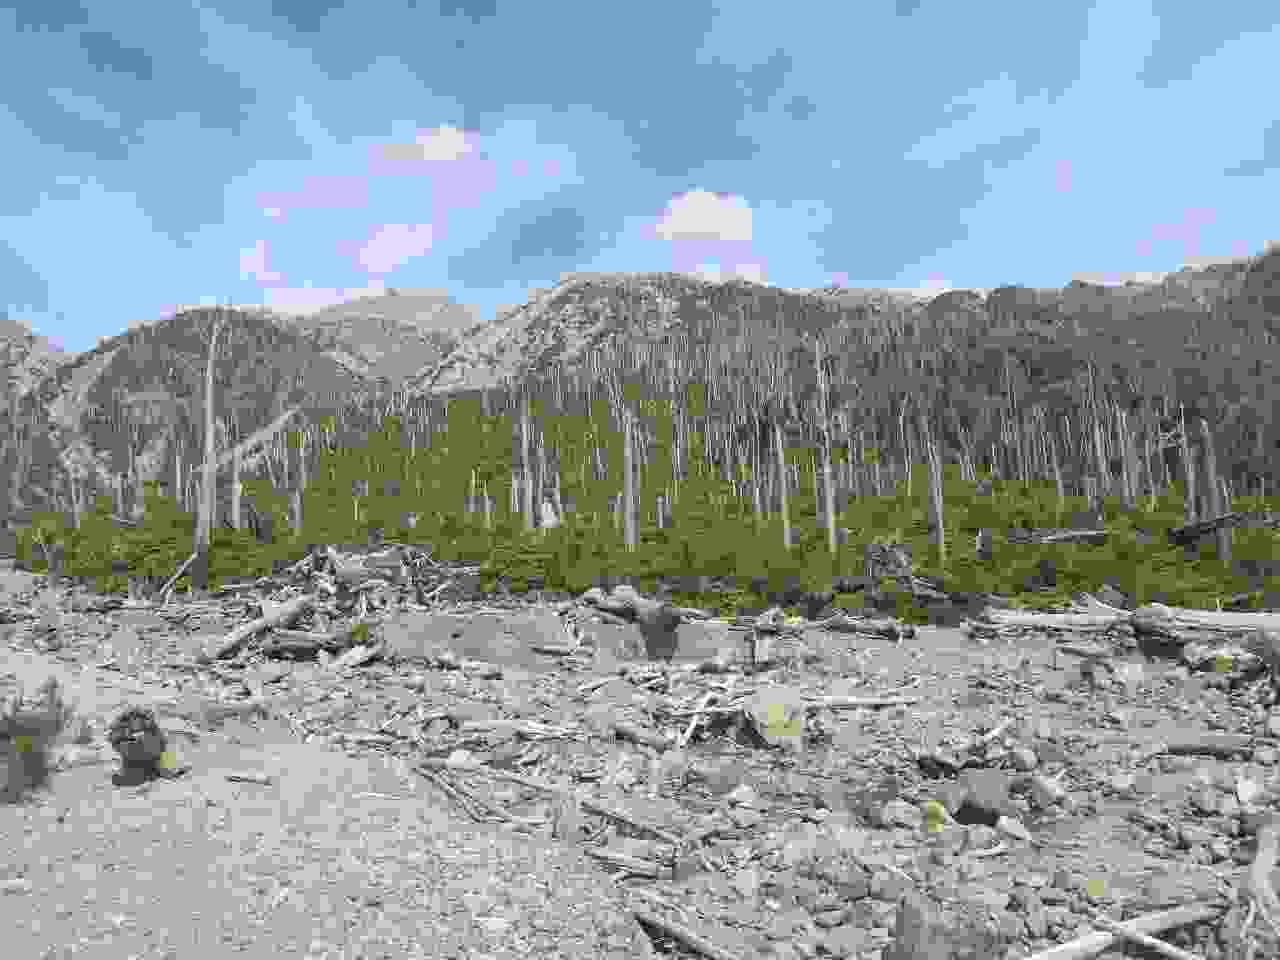
\includegraphics[height=90mm]{../wp-content/uploads/2015/02/P2222302.jpg} } 
  \newline
  \newline
\centerline{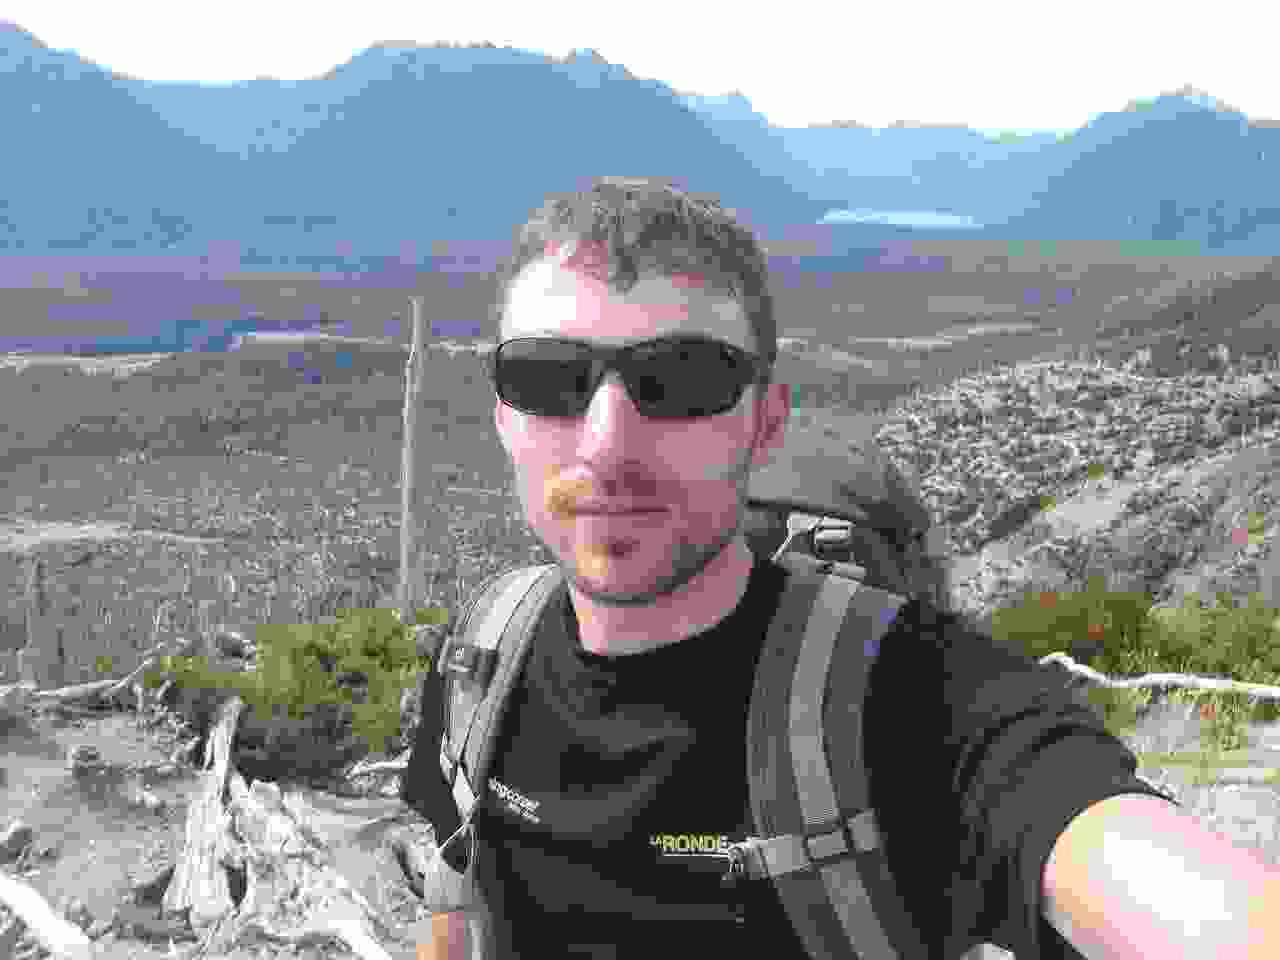
\includegraphics[height=90mm]{../wp-content/uploads/2015/02/P2222305.jpg} } 
 \newline
\centerline{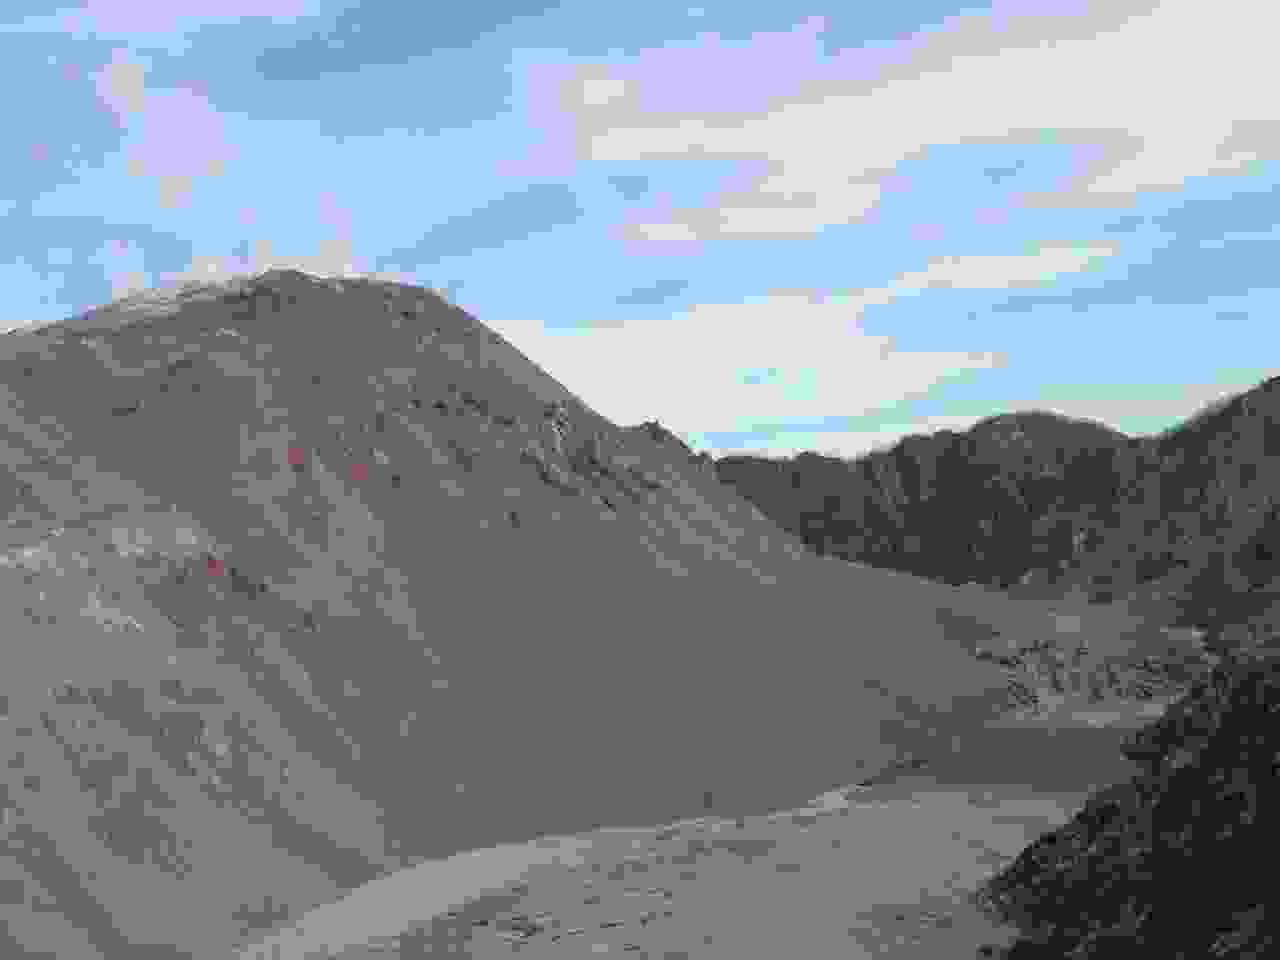
\includegraphics[height=90mm]{../wp-content/uploads/2015/02/P2222310.jpg} } 
 \newline
\centerline{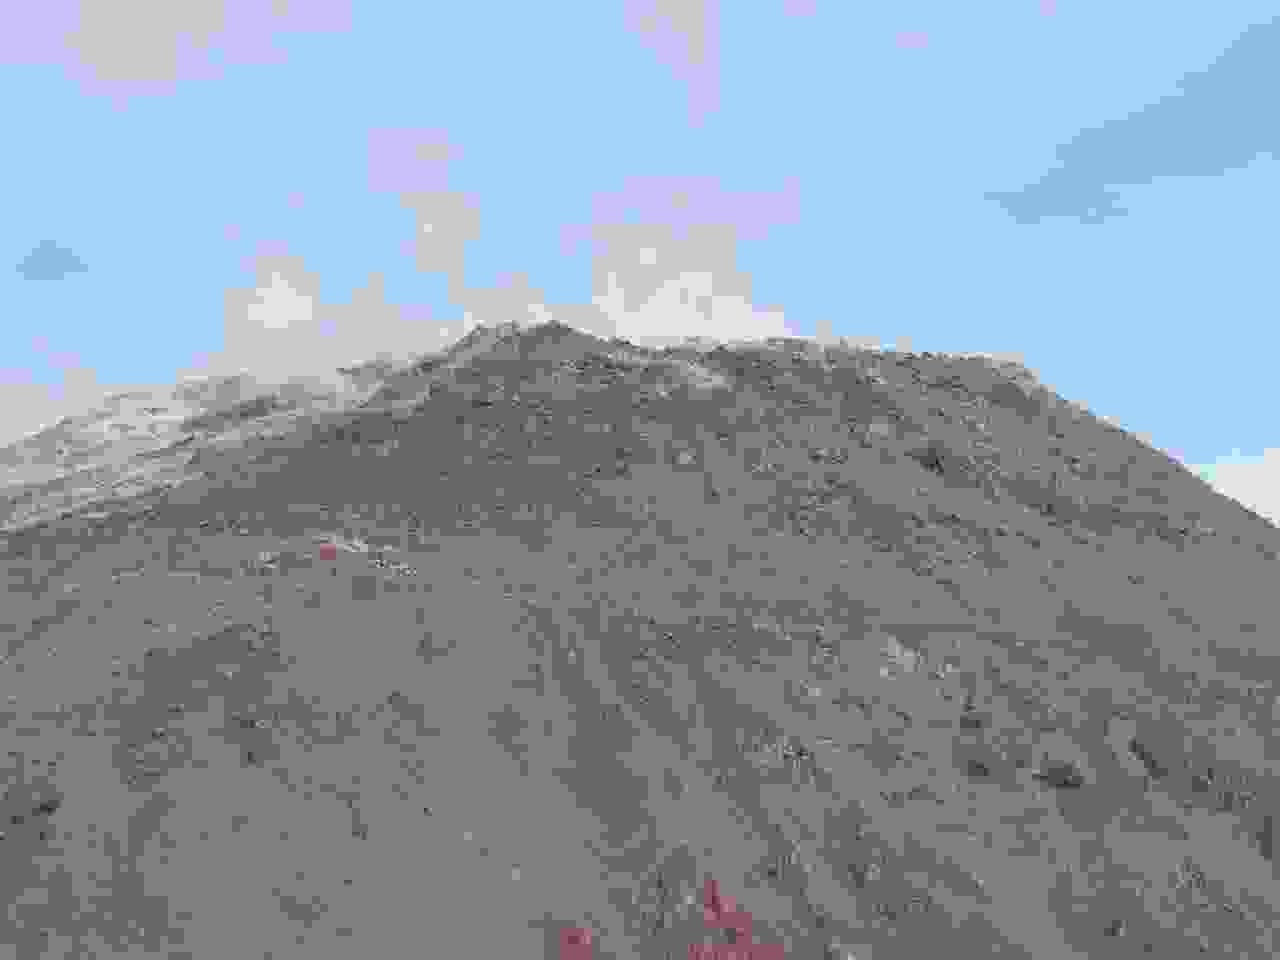
\includegraphics[height=90mm]{../wp-content/uploads/2015/02/P2222311.jpg} } 
 \newline
\centerline{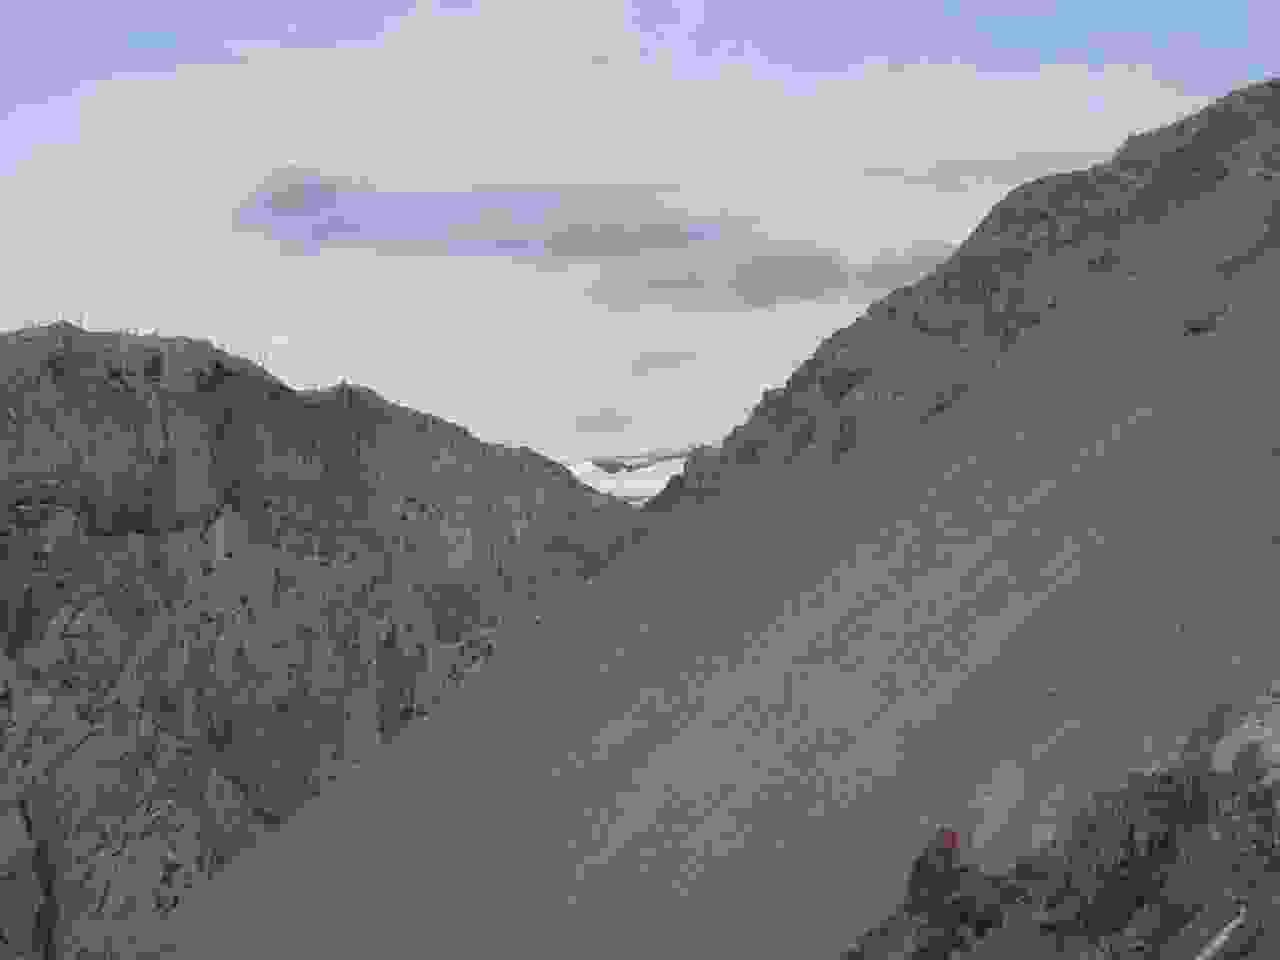
\includegraphics[height=90mm]{../wp-content/uploads/2015/02/P2222312.jpg} } 
Je continue direction Caleta Gonzalo, à l'intérieur du parc Pumalin. \newline
 \newline
\centerline{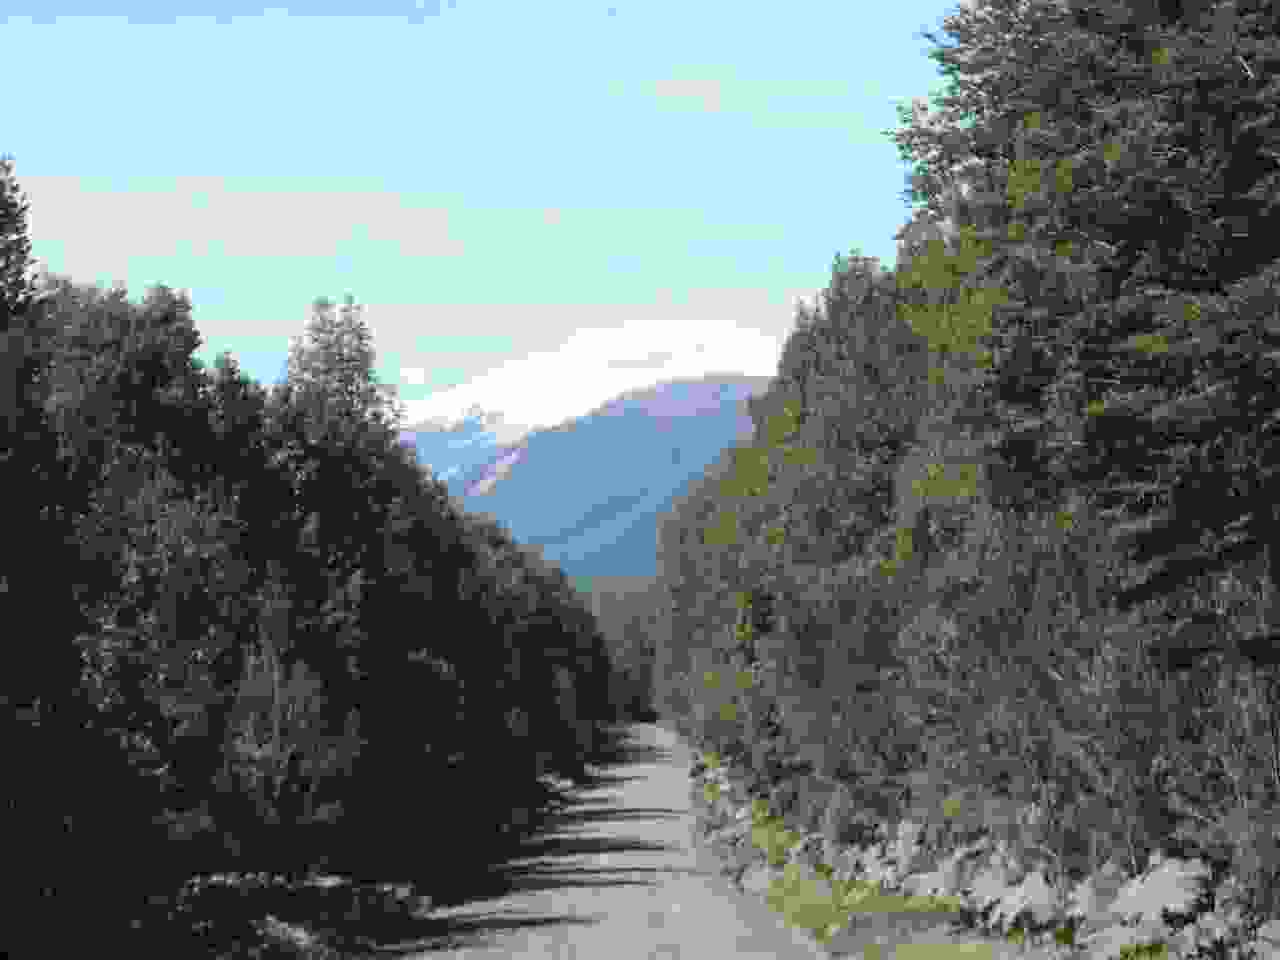
\includegraphics[height=90mm]{../wp-content/uploads/2015/02/P2222300.jpg} } 
 \newline
 \newline
\centerline{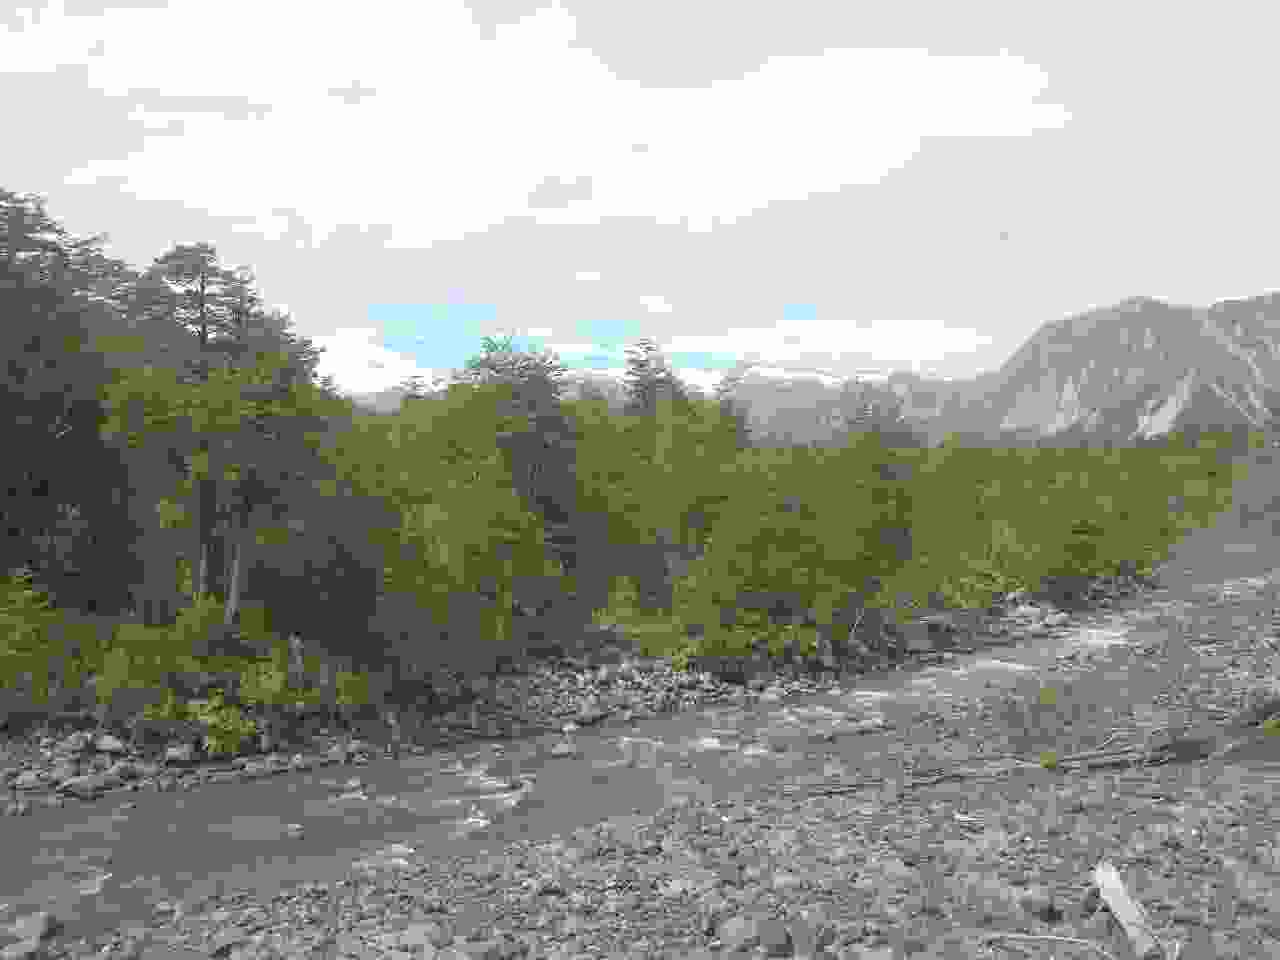
\includegraphics[height=90mm]{../wp-content/uploads/2015/02/P2232321.jpg} } 
 \newline
\centerline{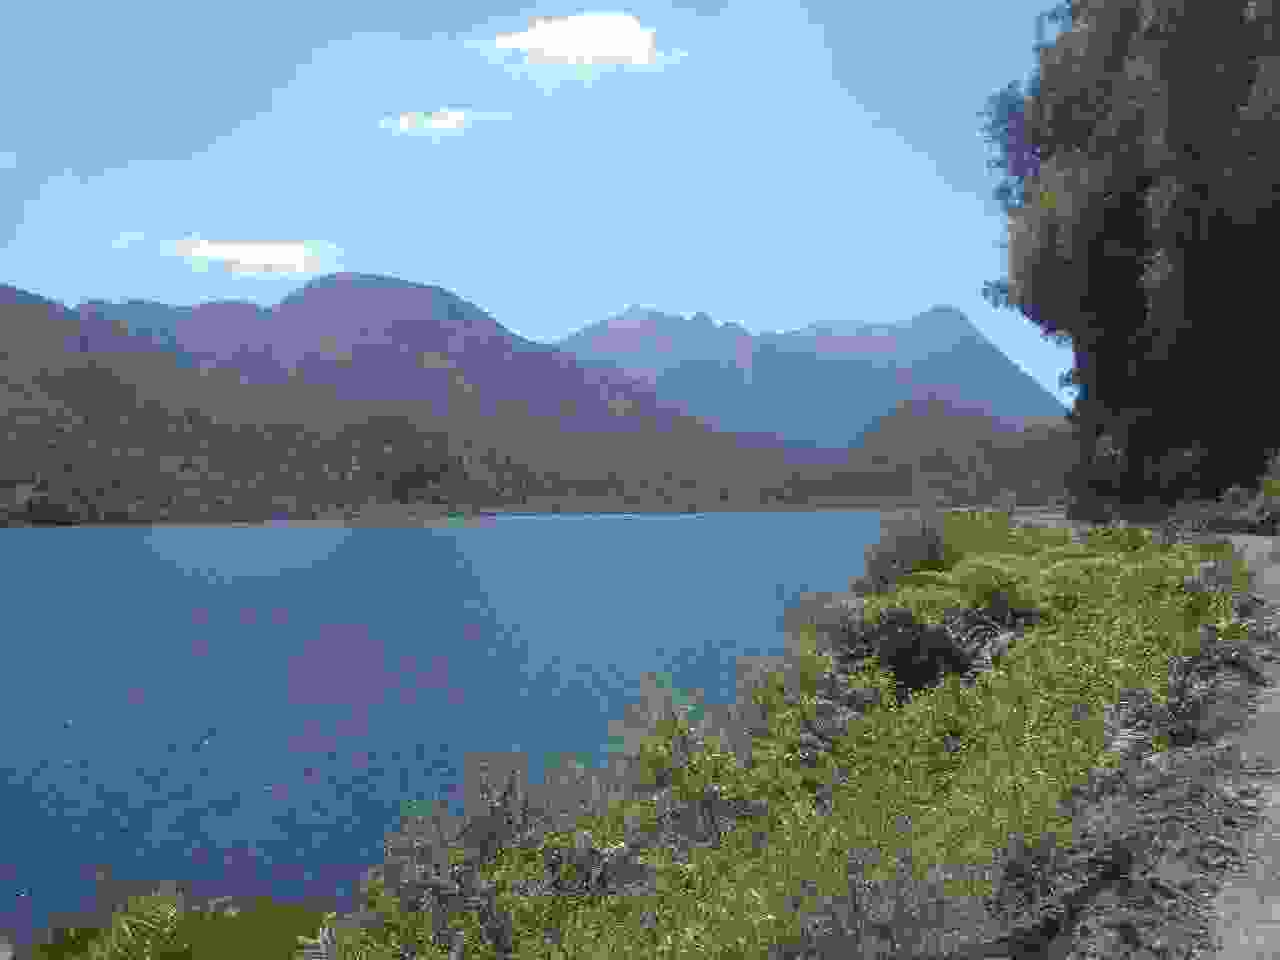
\includegraphics[height=90mm]{../wp-content/uploads/2015/02/P2232323.jpg} } 
 \newline
\centerline{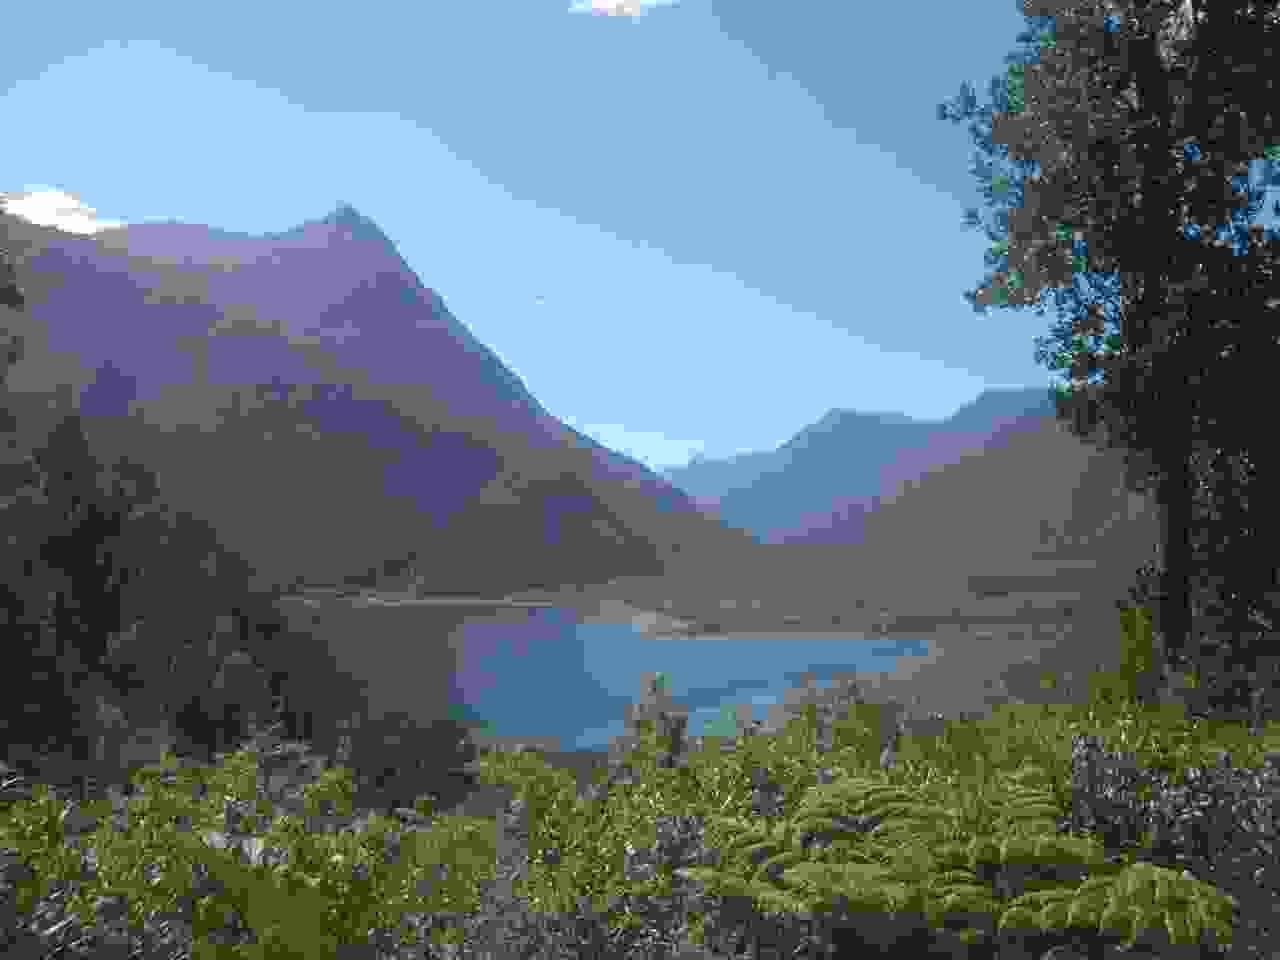
\includegraphics[height=90mm]{../wp-content/uploads/2015/02/P2232326.jpg} } 
 \newline
\centerline{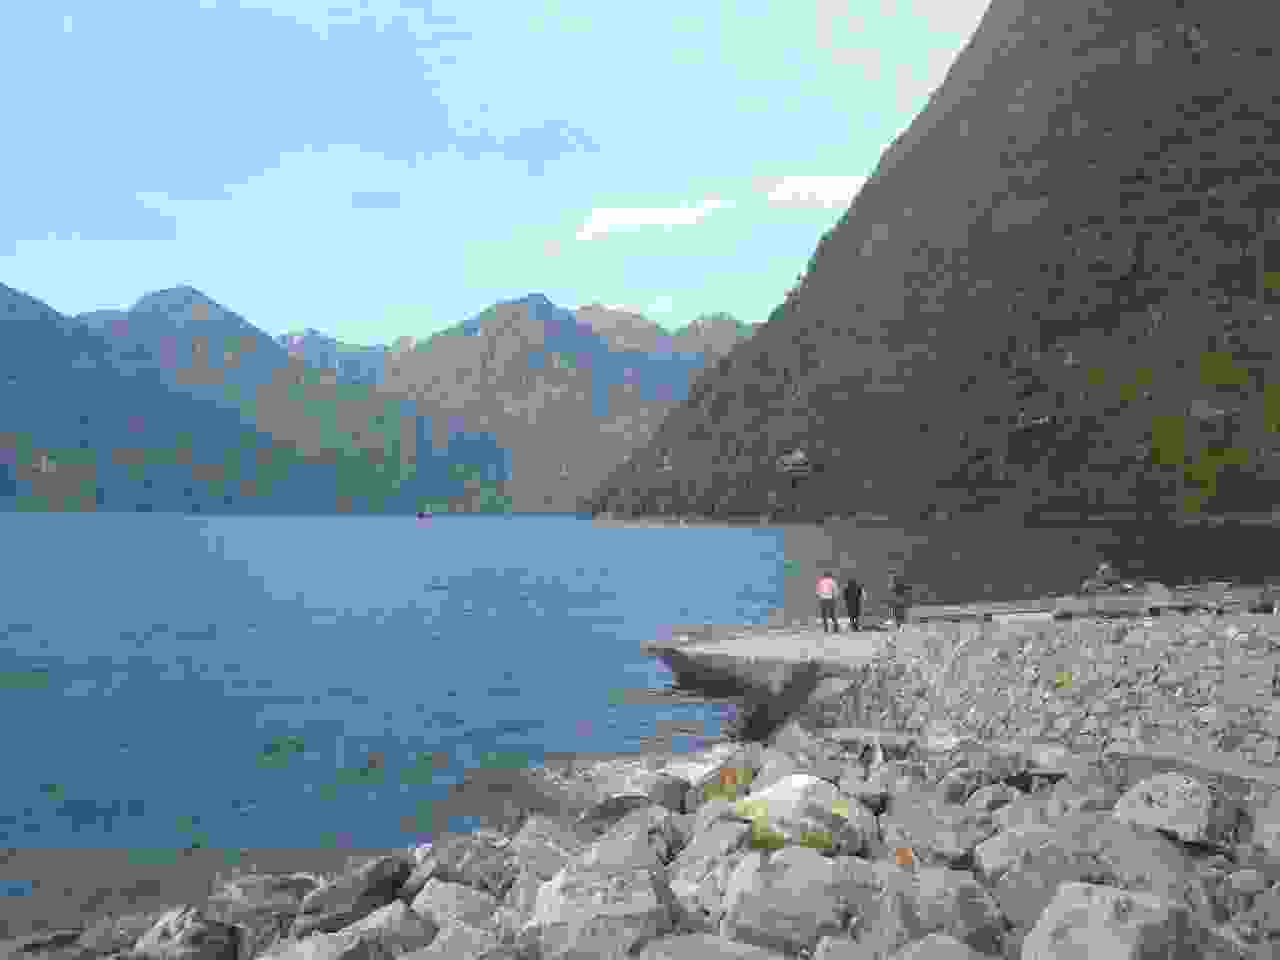
\includegraphics[height=90mm]{../wp-content/uploads/2015/02/P2232330.jpg} } 
 \newline
 Journée sur le ferry, encore magnifique entre fjords, montagnes et glaciers.\newline
\centerline{\includegraphics[height=90mm]{../wp-content/uploads/2015/02/P2242333.jpg} } 
 \newline
 \newline
\centerline{\includegraphics[height=90mm]{../wp-content/uploads/2015/02/P2242335.jpg} } 
 \newline
\centerline{\includegraphics[height=90mm]{../wp-content/uploads/2015/02/P2242338.jpg} } 
 \newline
\centerline{\includegraphics[height=90mm]{../wp-content/uploads/2015/02/P2242342.jpg} } 
 \newline
\centerline{\includegraphics[height=90mm]{../wp-content/uploads/2015/02/P2242345.jpg} } 
 \newline
\centerline{\includegraphics[height=90mm]{../wp-content/uploads/2015/02/P2242347.jpg} } 
 \newline
\centerline{\includegraphics[height=90mm]{../wp-content/uploads/2015/02/P2242348.jpg} } 
 \newline
\centerline{\includegraphics[height=90mm]{../wp-content/uploads/2015/02/P2242351.jpg} } 
 \newline
 \newline
\centerline{\includegraphics[height=90mm]{../wp-content/uploads/2015/02/P2242354.jpg} } 
\newline
\centerline{\includegraphics[height=90mm]{../wp-content/uploads/2015/02/P2242355.jpg} } 
 \newline
\centerline{\includegraphics[height=90mm]{../wp-content/uploads/2015/02/P2242358.jpg} } 
 \newline
\centerline{\includegraphics[height=90mm]{../wp-content/uploads/2015/02/P2242359.jpg} } 
 \newline
\centerline{\includegraphics[height=90mm]{../wp-content/uploads/2015/02/P2242363.jpg} } 
 \newline
\centerline{\includegraphics[height=90mm]{../wp-content/uploads/2015/02/P2242364.jpg} } 
 \newline
\centerline{\includegraphics[height=90mm]{../wp-content/uploads/2015/02/P2242366.jpg} } 
 \newline
\centerline{\includegraphics[height=90mm]{../wp-content/uploads/2015/02/P2252370.jpg} } 
Sur le bateau, j'ai rencontré un couple de français qui m'ont proposé de m'avancer en direction de Puerto Montt. Du coup je suis arrivé plus rapidement en évitant au passage une partie de piste en travaux qui aurait été galère. \newline
 J'en ai profité pour visiter le marché de poissons d'Angelmo. \newline
 \newline
\centerline{\includegraphics[height=90mm]{../wp-content/uploads/2015/02/P2252373.jpg} } 
 \newline
\centerline{\includegraphics[height=90mm]{../wp-content/uploads/2015/02/P2252372.jpg} } 
 \newline
 Saumon au beurre dans un des nombreux restaurants du marché. \newline
 \newline
\centerline{\includegraphics[height=90mm]{../wp-content/uploads/2015/02/P2252376.jpg} } 
 \newline
\centerline{\includegraphics[height=90mm]{../wp-content/uploads/2015/02/P2252375.jpg} } 
 \newline
 Passage par Puerto Varas au bord du lac Llanquihue, petite ville avec une architecture d'influence allemande. \newline
 \newline
\centerline{\includegraphics[height=90mm]{../wp-content/uploads/2015/02/P2252379.jpg} } 
 \newline
 Belle route le long du lac avec piste cyclable. \newline
 \newline
\centerline{\includegraphics[height=90mm]{../wp-content/uploads/2015/02/P2252386.jpg} } 
 \newline
\centerline{\includegraphics[height=90mm]{../wp-content/uploads/2015/02/P2252387.jpg} } 
 \newline
 Vues sur le volcan Osorno. \newline
 \newline
\centerline{\includegraphics[height=90mm]{../wp-content/uploads/2015/02/P2252385.jpg} } 
 \newline
 \newline
\centerline{\includegraphics[height=90mm]{../wp-content/uploads/2015/02/P2262390.jpg} } 
 \newline
\centerline{\includegraphics[height=90mm]{../wp-content/uploads/2015/02/P2262395.jpg} } 
Arrivée le lendemain aux chutes de Petrohué. \newline
 \newline
\centerline{\includegraphics[height=90mm]{../wp-content/uploads/2015/02/P2262401.jpg} } 
 \newline
\centerline{\includegraphics[height=90mm]{../wp-content/uploads/2015/02/P2262403.jpg} } 
 \newline
 C'est terminé pour le sud du Chili, prochaine étape Santiago puis l'île de Pâques. \newline
 \newline
\centerline{\includegraphics[height=90mm]{../wp-content/uploads/2015/02/P2282417.jpg} } 
 \newline
  \newline
  \newline
  \newline
  \newline
  \newline
  \newline
  \newline
  \newline
  \newline
  \newline
  \newline
  \newline
  \newline
  \newline
  \newline

\newpage
 
